\chapter{General Relativity - the Theory}

\label{ch:GRtheory}
\section{Introduction to General Relativity}
The experimentally well-established \emph{principle of equivalence}, stating the equivalence of inertial and gravitational mass, is the heuristic guiding principle of GR and has the following forms:
\begin{enumerate}
	\item The weaker and less precise statement is that the motion of a test body in a gravitational field is independent of its mass and composition.
	\item In a more precise form: In an arbitrary gravitational field no local non-gravitational experiment can distinguish a freely falling, non-rotating system from a uniformaly moving system in absence of the gravitational field $\rightarrow$ objects with different mass fall at the same speed under gravity.
\end{enumerate}

Where \emph{Freely falling frames of reference}:
It must be possible to introduce local, non-rotating, freely-falling frames of reference in which gravity is locally "transformed away".
The directions of motion of different freely-falling reference frames will generally not be parallel: E.g. Einstein elevators released at same height but different locations over Earth's surface.
\marginpar{A manifold with a metrix which is not positive definite is called pseudo-Riemannian, or Lorentzian if the metric has the signature of the Minkowski metric.}
\graffito{An outlook into the future of \texttt{classicthesis}.}
\subsection{Closer Look at the Equivalence Principle}
In other words:\\
The inertial mass clearly has a universal character, related to the resistance you feel when
you try to push on the object; it is the same constant no matter what kind of force is being
exerted 
\begin{equation}
\vec{f}=m_i \vec{a}.
\end{equation}
Gravitation on the other hand is
\begin{equation}
\vec{f}_G = -m_g \vec{\nabla} \Phi.
\end{equation}
On the face of it, $m_g$ has a very different character than $m_i$ ; it is a quantity specific to the
gravitational force. If you like, it is the “gravitational charge” of the body. Nevertheless,
Galileo long ago showed that the response of matter to gravitation was
universal — every object falls at the same rate in a gravitational field, independent of the
composition of the object.
\begin{mybox}{Weak Equivalence Principle}
In Newtonian mechanics this translates into the Weak Equivalence Principle (WEP), which is
simply
\begin{equation}
m_g = m_i
\end{equation}
for any object.
\end{mybox} 
An immediate consequence is that the behavior of freely-falling test particles
is universal, independent of their mass (or any other qualities they may have); in fact we have
\begin{equation}
\vec{a} =- \vec{\nabla} \Phi
\end{equation}
The WEP implies that there is no way to disentangle the effects of a gravitational field
from those of being in a uniformly accelerating frame, simply by observing the behavior of
freely-falling particles. This follows from the universality of gravitation; it would be possible
to distinguish between uniform acceleration and an electromagnetic field, by observing the
behavior of particles with different charges. But with gravity it is impossible, since the
“charge” is necessarily proportional to the (inertial) mass. To be careful, we should limit our claims about the impossibility of distinguishing gravity
from uniform acceleration by restricting our attention to “small enough regions of spacetime.”
The WEP can therefore be stated as “the laws of freely-falling particles are the same in a
gravitational field and a uniformly accelerated frame, in small enough regions of spacetime.”
In larger regions of spacetime there will be inhomogeneities in the gravitational field, which will lead to detectable tidal fields.
\\
\\
\begin{mybox}{Einstein Equivalence
	Principle, or EEP}
“In small enough regions of spacetime, the laws of physics reduce to
those of special relativity; it is impossible to detect the existence of a gravitational field."
\end{mybox}
\marginpar{Hence, $g\rightarrow\eta$ ?}
The EEP implies that gravity is inescapable — there is no such thing as a “gravitationally neutral
object” with respect to which we can measure the acceleration due to gravity. It follows
that “the acceleration due to gravity” is not something which can be reliably defined, and
therefore is of little use.
Instead, it makes more sense to \emph{define} “unaccelerated” as “freely falling,” and that is
what we shall do. This point of view is the origin of the idea that gravity is not a “force”
— a force is something which leads to acceleration, and our definition of zero acceleration is
“moving freely in the presence of whatever gravitational field happens to be around.”\\
The solution is to retain the notion of inertial frames, but to discard the hope that they
can be uniquely extended throughout space and time. Instead we can define \emph{locally inertial
	frames}, those which follow the motion of freely falling particles in small enough regions of
spacetime. This is the best we
can do, but it forces us to give up a good deal. For example, we can no longer speak with
confidence about the relative velocity of far away objects, since the inertial reference frames
appropriate to those objects are independent of those appropriate to us.
\subsection{Another look at the equivalence principle by Feynman}
\begin{statements} 
	The central idea of gravity, the most cogent fact about how it acts, is that weight and mass are exactly proportional, so that all objects accelerate under gravity at exactly the same rate, no matter what their constitution may be.
\end{statements}
The experiment of Eötvös showed how a centrifugal force added to a gravity force in such a way that the resultant was indistinguishable from a purely gravitational effect. The weightlessness in satellites is an example of a cancellation of gravitational forces by an acceleration. It is this possibility of cancellation which is the core of the principle of equivalence.\\
\\
In special relativity, extensive use is made of reference frames which are moving with a uniform velocity in a straight line. But, as soon as we allow the presence of gravitating masses anywhere in the universe, the concept of such truly unaccelerated motion becomes impossible, because there will be gravitational fields everywhere.\\
If we are performing experiments inside a box which is not in free fall, it will be possible to detect the presence of gravitation-like forces, by an experiment with masses coupled to springs for example. However, we cannot tell from inside the box whether we are accelerating relative to the nebulae, or whether the forces are due to masses in the neighbourhood:
\begin{mybox}{Equivalence principle, EP}
	It shall be impossible, by any experiment whatsoever performed inside such a box, to detect a difference between an acceleration relative to the nebulae and gravity. That is, an accelerating box in some gravitational field is indistinguishable from a stationary box in some different gravitational field.
\end{mybox}
\subsection{Consequences of principle of equivalence}
The principle of equivalence tells us that light falls in a gravitational field. If the box is accelerating, the light travels in a straight line in an unaccelerated system.\\
\\
The EP also tells us that clock rates are affected by gravity. Light which is emitted from the top of the accelerating box will look violet-shifted as we loom at it from the bottom. One way of describing this situation is to say that the time scale is faster at the top; time flows are diferent in different gravitational potentials, so that time flows are unequal in various parts of the world. How much is this time difference at various points in space ? To calculate it, we compare the time rates with an absolute time separation, defined i.t.o. the proper time $\md s$. Let us suppose that there are two events occuring at the top, which are reported to be a time $\md t$ apart; then
\begin{equation}
\phi = g h, \quad \md s = \md t(1 + \phi/c^2),
\end{equation}
in the limit of small velocities. The quantity $\phi$ is simply the potential difference between the location of the events, and the point of reference. A more careful computation gives us an expression good for all velocities 
\begin{equation}
\md s = \md t \sqrt{1+2 \phi/c^2}.
\end{equation}
\\
\\
\subsubsection{Equivalence Principle implies light deflection and gravitational redshift}
According to the equivalence principle, the downward gravitational acceleration felt in an
Einstein elevator cannot locally be distinguished from a constant upward acceleration of the
elevator with the same acceleration. Adopting the equivalence principle, one can thus assume
that the gravitational field is absent and that the elevator is constantly accelerated upward instead.
When the photon is received at the ceiling, the ceiling moves with a finite velocity compared to
the floor when the photon was emitted. The photon is thus Doppler shifted with respect to its
emission and is received with a longer wavelength.
\\
Note that Doppler shift in GR is defined by the change in frequency
\begin{equation}
\label{eq:dopplershiftgr}
\frac{\nu_s}{\nu_o} = \frac{g(k, u)|_s}{g(k, u)|_o},
\end{equation}
where $k$ is
the light’s four-wave vector, any distinction between Doppler shift and gravitational redshift has
no invariant meaning in general relativity.\\
Similarly, it can be concluded from the equivalence principle that light rays should be curved in
gravitational fields. Suppose that a horizontal light ray enters an Einstein elevator to the left and
leaves it at a later time to the right. As the light ray leaves the elevator, the elevator’s velocity
has increased so that in the rest frame of the elevator, it leaves at an angle downward from the
horizontal because of the aberration due to the finite speed of light.
\subsubsection{Equivalence Principle implies metric being a dynamical field}
The equivalence of inertial and gravitational mass led Einstein to the equivalence principle,
which says that it must be possible to introduce local, non-rotating, freely-falling frames of
reference in which gravity is locally “transformed away”. The directions of motion of different
freely-falling reference frames will generally not be parallel: Einstein elevators released at the
same height above the Earth’s surface but over different locations will fall towards the Earth’s
centre and thus approach each other. Replacing inertial frames by freely falling, non-rotating
frames of references leads to the idea that space-time is a four-dimensional manifold instead of
the “rigid”, four-dimensional Euclidean space.
In a freely-falling reference frame, special relativity must hold, implying that the Minkowskian
metric of special relativity must locally be valid. The same operation must be possible in all
freely-falling reference frames individually, but not globally. Thus, general relativity considers
the metric of the space-time manifold as a dynamical field.

\subsection{From Newton to Einstein}
 In
a significant change of perspective from regarding gravity as a force between point like
particles with mass, they instead follow straight lines through a curved geometry. Only
where these free-fall trajectories, or geodesics, cannot be sustained—for instance when the
surface of the Earth prevents us from falling through—do we experience a reaction. This
makes gravity locally indistinguishable from any inertial acceleration that we feel, for
instance, in an elevator accelerating upwards or in a car going around a corner. Closing
this reasoning, what induces the spacetime curvature in the theory of general relativity is
the matter and energy it carries. This makes even us slightly bend the spacetime around
us, so that objects and indeed also light are affected by our presence, and even more so
by more massive objects such as the planet Earth or the Sun.


\section{On our Path towards a curved Spacetime}
So far we have been talking strictly about physics, without jumping to the conclusion
that spacetime should be described as a curved manifold. It should be clear, however, why
such a conclusion is appropriate. The idea that the laws of special relativity should be
obeyed in sufficiently small regions of spacetime, and further that local inertial frames can
be established in such regions, corresponds to our ability to construct Riemann normal coordinates at any one point on a manifold — coordinates in which the metric takes its canonical
form and the Christoffel symbols vanish. The impossibility of comparing velocities (vectors)
at widely separated regions corresponds to the path-dependence of parallel transport on a
curved manifold. These considerations were enough to give Einstein the idea that gravity
was a manifestation of spacetime curvature.\\
\\
The principle of
equivalence tells us that the laws of physics, in small enough regions of spacetime, look like
those of special relativity. We interpret this in the language of manifolds as the statement
that these laws, when written in Riemannian normal coordinates $x^μ$ based at some point
$p$, are described by equations which take the same form as they would in flat space. The
simplest example is that of freely-falling (unaccelerated) particles. In flat space such particles
move in straight lines; in equations, this is expressed as the vanishing of the second derivative
of the parameterized path $x^μ (λ)$:
\begin{equation}
\frac{\md^2 x^\mu}{\md \lambda^2} = 0.
\end{equation}
According to the EEP, exactly this equation should hold in curved space, as long as the
coordinates $x^μ$ are RNC’s. What about some other coordinate system? As it stands, this is not an equation between tensors. However, there is a unique tensorial equation which
reduces to this when the Christoffel symbols vanish; it is the geodesic equation
\begin{equation}
\frac{\md^2 x^\mu}{\md \lambda^2} + \Gamma^\mu_{\rho \sigma} \frac{\md x^\rho}{\md \lambda} \frac{\md x^\sigma}{\md \lambda} = 0.
\end{equation}
In general relativity, therefore, free particles
move along geodesics; we have mentioned this before, but now you know why it is true.
\marginpar{General relativity keeps the light-cone structure of special relativity, even thought its rigidity is given up: the orientation of light cones can vary across space-time.}.

\section{Newtonian limit:}
We define the “\emph{Newtonian limit}” by
three requirements
\begin{enumerate}
\item the particles are moving slowly (with respect to the speed of light),
\item the gravitational field is weak (can be considered a perturbation of flat space),
\item the field is
also static (unchanging with time).
\end{enumerate}
Let us see what these assumptions do to the geodesic
equation, taking the proper time $τ$ as an affine parameter. “Moving slowly” means that
\begin{equation}
	\frac{\md x^i}{\md \tau} \ll \frac{\md t}{\md \tau}, 
\end{equation}
so the geodesic equation becomes
\begin{equation}
	\frac{\md^2 x^\mu}{\md \tau^2} + \Gamma^\mu_{00} \left(\frac{\md t}{\md \tau}\right)^2 = 0.
\end{equation}
Since the field is static, the relevant Christoffel symbols $Γ^μ_{00}$ simplify:
\begin{equation}
	\Gamma^\mu_{00} = \half g^{\mu \lambda} \left[\partial_0 g_{0\lambda} +\partial_0 g_{\lambda 0} - \partial_{\lambda}g_{00}\right]= - \half g^{\mu \lambda} \partial_{\lambda} g_{00}.
\end{equation}
Finally, the weakness of the gravitational field allows us to decompose the metric into the
Minkowski form plus a small perturbation:
\begin{equation}
	g_{\mu \nu} = \eta_{\mu \nu} +h_{\mu \nu}, \quad \abs{h_{\mu \nu}} \ll 1.
\end{equation}
(We are working in Cartesian coordinates, so $η\munu$ is the canonical form of the metric. The
“smallness condition” on the metric perturbation $h_{μν}$ doesn’t really make sense in other
coordinates.) From the definition of the inverse metric, $g_{μν} g^{νσ} = δ^σ_μ$ , we find that to first
order in $h$,
\begin{equation}
	g^{\mu \nu} = \eta^{\mu \nu} -h^{\mu \nu} .
\end{equation}
where $h^{μν} = η^{μρ} η^{νσ} h_{ρσ}$ . In fact, we can use the Minkowski metric to raise and lower indices
on an object of any definite order in $h$, since the corrections would only contribute at higher
orders.\\
Putting it all together, we find
\begin{equation} 
\Gamma^\mu_{00} = -\half \eta^{\mu \lambda} \partial_{\lambda} h_{00}.
\end{equation}
Inserting into our form of the geodesic equation we thus find
\begin{equation}
	\frac{\md^2 x^\mu}{\md \tau^2} = \half \eta^{\mu \lambda} \partial_{\lambda} h_{00} \left(\frac{\md t}{\md \tau}\right)^2.
\end{equation}
Using $∂_0 h_{00} = 0$, the $μ = 0$ component of this is just
\begin{equation}
	\frac{\md^2 t}{\md \tau^2} = 0.
\end{equation}
That is, $\frac{\md t}{\md \tau}$
is constant. To examine the spacelike components, recall that the
spacelike components of $η_{μν}$ are just those of a $3 × 3$ identity matrix. We therefore have
\begin{equation}
	\frac{\md^2 x^i}{\md \tau^2} = \half \left(\frac{\md t}{\md \tau}\right)^2 \partial_0 h_{00}.
\end{equation}
Dividing both side by $\left(\frac{\md t}{\md \tau}\right)$ has the effect of converting the derivative on the LHS from $\tau$ to $t$, leaving us with
\begin{equation}
	\frac{\md^2 x^i}{\md t^2} = \half \partial_i h_{00}.
\end{equation}
This begins to look a great deal like Newton’s theory of gravitation. In fact, if we compare
this equation to $\vec{a}=-\vec{\nabla} \Phi$, we find that they are the same once we identify
\begin{equation}
	h_{00} = -2 \Phi,
\end{equation}
or in other words
\begin{equation}
	g_{00} = -(1+2 \Phi).
\end{equation}
Therefore, we have shown that the curvature of spacetime is indeed sufficient to describe
gravity in the Newtonian limit, as long as the metric takes this form.

\section{General Covariance}
\label{sec:generalcovariance}
One could always proceed and calculate general physical laws as we did in the derivation of the geodesic equation via Weinberg and start of in RNC and then transform to general laboratory coordinate system, but this is tedious. Instead, we shall follow a different method, one that is of precisely the same physical content, but is much more elegant in appearance and convenient in execution. This method is based on an alternative version of the Principle of Equivalence, known as
\begin{mybox}{Principle of General Covariance}
	...the \emph{Principle of General Covariance}. It states that a physical equation holds in a general gravitational field if two conditions are met:
	\begin{enumerate}
		\item[(1)] The equation holds in the absence of gravitation; that is, it agrees with the laws of special relativity when the metric tensor $g_{\alpha \beta}$ equals the Minkowskian tensor $\eta_{\alpha \beta}$ and when the affine connection coefficients $\Gamma^\alpha_{\beta \gamma}$ vanish.
		\item[(2)] The equation is generally covariant; that is, it preserves its form under a general coordinate transformation $x\rightarrow x^\prime$.
	\end{enumerate}
\end{mybox}
To see that the Principle of General Covariance follows from the Principle of Equivalence, let us suppose that we are in an arbitrary gravitational field, and consider any equation that satisfies the two above conditions. From (2), we learn that the equation will be true in all coordinate systems if it is true in any one coordinate system. But at any point there is a class of coordinate systems, the locally inertial systems, in which the effects of gravitation are absent. Condition (1) then tells us that our equation holds in these systems, and hence in all other coordinate systems.\\
The significance of the Principle of General Covariance lies in its statement about the effects of gravitation, that a physical equation by virtue of its general covariance will be true in a gravitational field if it is true in the absence of gravitation, general covariance by itself has no physical content.
\begin{mybox}{Comparison of general covariance with Lorentz invariance}
	Just as any equation can be made generally covariant, so any equation can be made Lorentz-invariant. However, if we do the latter with a nonrelativistic eq. like Newton II, we find after making it Lorentz-invariant that a new quantity has entered the equation, which of course is the velocity of the coordinate frame w.r.t. the original reference frame. The requirement that this velocity \emph{not} appear in the transformed equation is called Principle of Special Relativity, or \emph{Lorentz invariance.}  \\
	Similarly, when we make an eq. covariant, the metric tensor and Christoffels enter the equation. The difference is that we do not require that these quantities drop out at the end, and hence we do not obtain any restrictions on the equation we start with; rather, we \emph{exploit the presence of $g\munu$ and $\Gamma^\lambda\munu$} to represent gravitational fields. In other words:
	\begin{statements}
		The Principle of General Covariance is \textbf{not} an invariance principle, like the Principle of Galilean, or Special Relativity, but is instead a statement about the effects of gravitation, and about nothing else. \textbf{In particular, general covariance does not imply Lorentz invariance}.
	\end{statements}
\end{mybox}
Any physical principle, such as general covariance, which takes the form of an invariance principle, but whose content is actually limited to a restriction on the interactions of one particular field, is called a \emph{dynamic symmetry}. There are other dynamic symmetries of importance in physics, such as local gauge invariance, which governs the interactions of the electromagnetic field, and chiral symmetry.\\
\\
The Principle of General Covariance can only be applied on a scale that is small compared with the space-time distances typical of the gravitational field, for it is only on this small scale that we are assured by the Principle of Equivalence of being able to construct a coordinate system in which the effects of gravitation are absent.\\
\\
Since we only apply the Principle of General Covariance on a small scale compared with the scale of the gravitational field, we usually expect that it is only $g\munu$ and its first derivatives that enter our generally covariant equations. \emph{This is precisely what we need to construct the Einstein-Hilbert action solely from the Ricci scalar, thus assume Principle of General Covariance and we can then postulate that the invariant scalar of the theory should only depend on the metric and its first derivatives.}
\\Thus, General covariance is not an ordinary symmetry principle like Lorentz invariance, but is rather a dynamical principle that governs the effect of gravitational fields.\\
\\
Caroll describes it like this, just use as a source of intuition, Weinberg above is correct:\\
Our next task is to show how the remaining laws of physics, beyond those governing freely-
falling particles, adapt to the curvature of spacetime. The procedure essentially follows the
paradigm established in arguing that free particles move along geodesics. Take a law of
physics in flat space, traditionally written in terms of partial derivatives and the flat metric.
According to the equivalence principle this law will hold in the presence of gravity, as long
as we are in Riemannian normal coordinates. Translate the law into a relationship between
tensors; for example, change partial derivatives to covariant ones. In RNC’s this version of
the law will reduce to the flat-space one, but tensors are coordinate-independent objects, so
the tensorial version must hold in any coordinate system.\\
This procedure is sometimes given a name, the \emph{Principle of Covariance}. I’m not
sure that it deserves its own name, since it’s really a consequence of the EEP plus the
requirement that the laws of physics be independent of coordinates. (The requirement that
laws of physics be independent of coordinates is essentially impossible to even imagine being
untrue. Given some experiment, if one person uses one coordinate system to predict a result
and another one uses a different coordinate system, they had better agree.).\\
We have already implicitly used the principle of covariance (or whatever you want to
call it) in deriving the statement that free particles move along geodesics.



\subsection{Principle of General Covariance represented by Diffeomorphism Invariance in GR}
The theory is coordinate invariant. Although such a statement
is true, it is a source of great misunderstanding, for the simple fact that it conveys very little
information. Any semi-respectable theory of physics is coordinate invariant, including those
based on special relativity or Newtonian mechanics; GR is not unique in this regard. When
people say that GR is diffeomorphism invariant, more likely than not they have one of two
(closely related) concepts in mind: the theory is free of “prior geometry”, and there is no
preferred coordinate system for spacetime. The first of these stems from the fact that the
metric is a dynamical variable, and along with it the connection and volume element and
so forth. Nothing is given to us ahead of time, unlike in classical mechanics or SR. As
a consequence, there is no way to simplify life by sticking to a specific coordinate system
adapted to some absolute elements of the geometry. This state of affairs forces us to be very
careful; it is possible that two purportedly distinct configurations (of matter and metric)
in GR are actually “the same”, related by a diffeomorphism. In a path integral approach
to quantum gravity, where we would like to sum over all possible configurations, special
care must be taken not to overcount by allowing physically indistinguishable configurations
to contribute more than once. In SR or Newtonian mechanics, meanwhile, the existence
of a preferred set of coordinates saves us from such ambiguities. The fact that GR has no
preferred coordinate system is often garbled into the statement that it is coordinate invariant
(or “generally covariant”); both things are true, but one has more content than the other.
On the other hand, the fact of diffeomorphism invariance can be put to good use. 
\subsubsection{Mathematical Viewpoint of General Covariance $=$ Diffeomorphism Invariance}

\begin{mybox}{Diffeomorphism invariance}
	Let $\phi$ be a diffeomorphism of $M$, such that $\phi:M\rightarrow N$ in diffemorphic way. Since $\phi$ is then bijective and smoothly differentiable and has a smoothly differentiable inverse, $M$ and $N$ can be considered as indistinguishable abstract manifolds. The manifolds $M$ and $N$ then represent the same physical space-time. In particular, the metric $g$ on $M$ is then physically equivalent to the pulled-back metric $\phi^* g$. The diffeomorphism invariance is a fundamental property of GR.\\
	\\
	This implies that coordinate systems don't have a physical significance.
\end{mybox}

It has the following equivalent interpretations or implications:\\
\begin{enumerate}
	\item Invariance of the form of physical laws under arbitrary differentiable coordinate transformations. The essential idea is that coordinates do not exist \emph{a priori} in nature, but are only artifices used in describing nature, and hence should play no role in the formulation of fundamental physical laws.
	\item Active POV: $g\rightarrow \phi^* g$ leaves the physics invariant vs. \\
	Passive POV: diffeomorphism invariance $\Leftrightarrow$ coordinate invariance.
	\item Diffeomorphism invariance $\Rightarrow$ invariance under specific class of gauge transformations:\\
	Let $\phi_t$ represent local flow of $f$ of vector field $v$, then
	\begin{equation}
	g \rightarrow \phi^* g = g + t \mathcal{L}_v g + \mathcal{O}(t^2).
	\end{equation}
\end{enumerate}


\subsubsection{Implications of Diffeomorphism invariance}
Recall
that the complete action for gravity coupled to a set of matter fields $ψ^i$ is given by a sum of
the Hilbert action for GR plus the matter action,
\begin{equation}
S = \frac{c^4}{8 \pi \mathcal{G}} S_{EH} [g_{\mu \nu}] +S_M[\psi^i,g_{\mu \nu}].
\end{equation}
The Hilbert action $S_{EH}$ is diffeomorphism invariant when considered in isolation, so the matter
action $S_M$ must also be if the action as a whole is to be invariant. We can write the variation
in $S_M$ under a diffeomorphism as
\begin{equation}
\delta S_M =  \int \md^n x \frac{\delta S_M}{\delta g_{\mu \nu}} \delta g_{\mu \nu} + \int \md^n x \frac{\delta S_M}{\delta \psi^i} \delta \psi^i.
\end{equation}
We are not considering arbitrary variations of the fields, only those which result from a
diffeomorphism. Nevertheless, the matter equations of motion tell us that the variation of
$S_M$ with respect to $ψ^i$ will vanish for any variation (since the gravitational part of the action
doesn’t involve the matter fields). Hence, for a diffeomorphism invariant theory the first
term on the right hand side must vanish. If the diffeomorphism is generated by a
vector field $V^μ (x)$, the infinitesimal change in the metric is simply given by its Lie derivative
along $V^μ$ ; thus with \ref{eq:liederivMetric}
\begin{equation}
\delta g_{\mu \nu} = \mL_V g_{\mu \nu} = 2 \nabla_{(\mu} V_{\nu)} .
\end{equation}
Setting $\delta S_M=0$ then implies
\begin{equation}
0=\int \md^n x \frac{\delta S_M}{\delta g_{\mu \nu}} \nabla_\mu V_\nu = - \int \md^n x\sqrt{-g} V_\nu \nabla_\mu \left(\frac{1}{\sqrt{-g}} \frac{\delta S_M}{\delta g_{\mu \nu}}\right),
\end{equation}
where we are able to drop the symmetrization of $∇_{(μ} V_{ ν)}$ since $δS_M /δg_{μν}$ is already symmetric.\\
\begin{mybox}{Energy-momentum conservation by diffeomorphism invariance of GR}
	Demanding that this should hold for diffeomorphisms generated by arbitrary vector fields $V_μ$ , and
	using the definition \ref{eq:GRenergymomentumtensor} of the energy-momentum tensor, we obtain precisely the law of
	energy-momentum conservation,
	\begin{equation}
	\nabla_\mu T^{\mu \nu} =0.
	\end{equation}
	This is why we claimed earlier that the conservation of $T_{μν}$ was more than simply a consequence of the Principle of Equivalence; it is much more secure than that, \emph{resting only on the
		diffeomorphism invariance of the theory.}
	
\end{mybox}



\subsection{The physical meaning of curvature}
\begin{mybox}{Tidal field and curvature}
	The curvature represents the gravitational tidal field, describing the relative acceleration of freely-falling test bodies, with the GR $\leftrightarrow$ Newtonian correspondences
	\begin{equation}
	\bar{R}^i_{0j0} \leftrightarrow \frac{\partial_i \partial_j \Phi}{c^2}, \qquad R_{\mu \nu} u^{\mu} u^{\nu} \leftrightarrow \frac{\vec{\nabla}^2 \Phi}{c^2}.
	\end{equation}
	Comparing the equation of geodesic deviation with the acceleration of two test bodies separated
	by a certain distance in Newtonian gravity shows that the curvature represents the gravitational
	tidal field, describing the relative accelerations of freely-falling test bodies.
\end{mybox}
\subsubsection{Gravitation versus Curvilinear Coordinates}
Suppose that we are presented with a metric tensor $g\munu(x)$ that is not just a constant. How can we tell if the space is really permeated by a gravitational field, or if $g\munu$ merely represents the metric $\eta_{\alpha \beta}$ of special relativity written in curvilinear coordinates ? In other words, how can we tell whether there is a set of Minkowskian coordinates $\xi^\alpha(x)$ that everywhere satisfy the condition
\begin{equation}
	\label{eq:MinkowskiToGRmetric}
	\eta^{\alpha \beta} = g^{\mu \nu} \frac{\partial \xi^\alpha(x)}{\partial x^\mu} \frac{\partial \xi^\beta(x)}{\partial x^\nu}.
\end{equation}
Note that the equivalence principle only says that at every point $X$ we can find locally inertial coordinates $\xi_X(x)$ that satisfy \ref{eq:MinkowskiToGRmetric} in an infinitesimal neighbourhood of $X$; what we are asking now is whether we can find one set of coordinates $\xi^\alpha(x)$ that satisfy \ref{eq:MinkowskiToGRmetric} everywhere. For example, the metric coefficients
\begin{equation}
	g_{rr}=1,\; g_{\theta \theta}=r^2, \; g_{\varphi \varphi}= r^2 \sin^2 \theta, \; g_{tt} =-1
\end{equation}
we know that there is a set of $\xi^\alpha$s satisfying \ref{eq:MinkowskiToGRmetric}, that is,
\begin{equation}
	\xi^1=r \sin \theta \cos \varphi , \; \xi^2 = r \sin\theta \sin \varphi, \; \xi^3 = r\cos \theta, \; \xi^4 = t
\end{equation}
but how could we have known that the given $g\munu$ was really equivalent to the Minkowski metric $\eta_{\mu \nu}$, if we weren't clever enoguh to have recognized it as simply $\eta_{\alpha \beta}$ in spherical polar coordinates?\\
The answer is contained in the following theorem
\begin{mybox}{General metric to Minkowski metric -  Truly flat space}
	The necessary and sufficient conditions for a metric $g\munu(x)$ to be equivalent to the Minkowski metric $\eta_{\alpha \beta}$ [in the sens that there is a transformation $x\rightarrow \xi$ satisfying \ref{eq:MinkowskiToGRmetric}] are, first that the curvature tensor calculated from $g\munu$ must \emph{everywhere} vanish,
	\begin{equation}
		\bar{R}^\lambda_{\mu\nu\kappa}=0
	\end{equation}
	and, second, that at some point $X$ the matrix $g^{\mu \nu}(X)$ has thee positive and one negative eigenvalue.
\end{mybox}
Another way to see that the Riemann tensor expresses the presence or absence of a true gravitational field is via the commutation of covariant derivative:
\begin{equation}
	V^\lambda_{;\nu;\kappa} - V^\lambda_{\;\kappa;\nu} = V^\sigma \bar{R}^\lambda_{\sigma \nu \kappa}.
\end{equation}
Thus, if the curvature tensor vanishes, then covariant derivatives \emph{commute}, as would be expected for a coordinate system that can be transformed into a Minkowski coordinate system.

\subsubsection{The Geometric Analogy}
We have seen that the non-vanishing of the tensor $\bar{R}_{\mu \nu \lambda \kappa}$ is the true expression of the presence of a gravitational field. It is therefore not surprising that Einstein and his successors have regarded the effects of a gravitational field as producing a change in the geometry of space and time. At one time it was even hoped that the rest of physics could be brought into a geometric formulation, but this hope has met with disappointment, and the geometric interpretation of the theory of gravitation has dwindled to a mere analogy, which lingers in our language in terms like "metric", "affine connection coefficients", and "curvature," but is not otherwise very useful. The important thing is to be able to make predictions about images on the astronomers' photographic plates etc. and it simply doesn't matter whether we ascribe these predictions to the physical effect of gravitational fields on the motion of planets and photons or to a curvature of space and time.\\


































\newpage

\section{Physical laws in external gravitational fields - Thus a metric is given, what are the dynamics}

\subsection{Relativistic variational principle}
The requirement that the proper time should be a maximum is equivalent to the principle of least action in the classical limit. This result suggests how we might obtain a mechanical principle (equivalent roughly to Newton's Second Law) which will be relativistic. It is that the variation of the length functional should be zero
\begin{equation}
\delta  \int_1^2 \md s=0.
\end{equation}
This principle will give the motion in the presence of gravitational fields, i.e. the geodesic equation. This solved the problem of finding the equations of motion given the field. The question before Einstein was now how to get the correct $\phi$, which is contained in $\md s$.It was Einstein's guess that in situations such as these, it should not matter whether we use the universally correct $\phi$ or not; if this $\phi$ is correctly defined, the description of the physics should be independent of the particular way in which we have separated inertial and gravitational effects, i.e. $\md s^2 = g\munu \md x^\mu \md x^\nu$ generally.
\subsection{Proper time in general coordinates}
The complete description of gravity can always be specified by a metric tensor $g\munu$ such that
\begin{equation}
\md s^2 = g\munu \md x^\mu \md x^\nu.
\end{equation}
The case of zero field corresponds to a particularly simple form for the metric tensor,$g\munu = \eta\munu$. As we change the coordinate system, the new metric tensor is given by
\begin{equation}
g^\prime_{\alpha \beta} = \frac{\partial x^\mu}{\partial x^{\alpha^\prime}} \frac{\partial x^\nu}{\partial x^{\beta^\prime}} g\munu.
\end{equation}
As before, the motion of particles is given by the requirement that the proper time is to be a maximum. If it is possible, by some kind of judicious choice of transformation, to reduce the tensor so that $g^\prime_{\alpha \beta} = \eta_{\alpha \beta}$, then we may conclude that \emph{there is no gravitational field} (compare EEP in intro), and that there is no acceleration. But this cannot be done in general, since the general tensor $g\munu$ represents ten presumably independent function, and only four functions can be specified in the transformation of coordinates. Only under very special circumstances can accelerations transform away all the $g\munu$ everywhere, i.e. RNC. If there really is some matter in the environment, then the reduction to $\eta\munu$ will be impossible. In that case all possible tensors $g\munu$ related by the above transformation equation will be equivalent, since non of them will lead to particularly simple expressions for $\md s^2$.
\\
\\
What we have achieved is to learn something of the character of the description of gravitational forces. In Newtonian theory, the corresponding thing is the statement that the force is given by the gradient of a scalar function.
\begin{align}
	\mathrm{Newtonian\, Gravity}: \; m\ddot{x} &= F_x, \quad F_x = - \nabla \phi,\\
	\mathrm{Einstein \, Theory}: \delta \int \md s &= 0, \quad \md s^2 = g\munu \md x^\mu \md x^\nu.
\end{align}
The second part of the theory corresponds to the specification of how the potential ($\phi$ or $g\munu$)   are related to matter. In the Newtonian theory we have
\begin{equation}
\laplacian{\phi} = 4\pi \mG \rho.
\end{equation}
We shall eventually arrive at a specification of the tensor $g\munu$ in terms of the matter. \\
The central idea is that since matter is physical, whereas coordinate systems are not, matter must be described in such a way that the results of solving the e.o.m. are independent of the particular choice of coordinates - the meaningful properties of the tensor $g\munu$ are expected to be invariant quantities under arbitrary transformations.

\subsection{Motion of particles}
Parametrize the trajectory of a particle as a curve $\gamma(\tau)$ with $\md x = \dot{\gamma} \md \tau$. The free action of a particle, with $\md \tau c = \md s$, is
\begin{equation}
S = - mc^2 \int_a^b \md \tau = -mc \int_a^b \sqrt{-g(\dot{\gamma},\dot{\gamma}) \md \tau} = -mc \int_a^b \sqrt{-\langle \dot{\gamma}, \dot{\gamma} \rangle}.
\end{equation}
The negative sign under the root comes about since the curve has to be timelike.
\begin{mybox}{Motion of freely falling particles}
	The trajectories extremizing this action are geodesic curves. Freely falling particles thus follow geodesics of the space-time.
\end{mybox}
This comes about since the extermization of the action given above results in the geodesic equation.\\
Note, if you define $c \md \tau = \sqrt{-\md s^2} \Rightarrow \rangle u,u \rangle = -c^2$,\\
but if you define $\md \tau = \sqrt{-\md s^2} \rightarrow \langle u,u \rangle = -1$.
$\md s^2$ is invariant under transformations generally, since we are only performing isometric transformations.





\subsection{Motion of light}
\marginpar{Ambiguities may occur when second derivatives are around, start substitution at beginning not at the end}
\marginpar{The problem of ordering
	covariant derivatives is similar to the problem of operator-ordering ambiguities in quantum
	mechanics.}
The importance of covariant differentiation arises from two of its properties:\\
It converts tensors to other tensors, and it reduces to ordinary differentiation in the absence of gravitation, that is, when $\Gamma^\mu_{\nu \lambda}=0$. These properties suggest the following algorithm for assessing the effects of gravitation on physical systems:\\
\emph{Write the appropriate special-relativistic equations that hold in the absence of gravitation, replace $\eta\munu$ with $g\munu$, and replace all derivatives with covariant derivatives}. The resulting equations will be generally covariant and true in the absence of gravitation, and therefore, according to the Principle of General Covariance, they will be true in the presence of gravitational fields, provided always that we work on a space-time scale sufficiently small compared with the scale of the gravitational field.
\begin{mybox}{Porting physical laws into general relativity}
	In the presence of a gravitational field, the physical laws of special realtivity are changed simply by substituting the covariant derivative for the partial derivative, $\partial \rightarrow \nabla$, by raising indices with $g^{\mu \nu}$ instead of $\eta^{\mu \nu}$ and by lowering them with $g_{\mu \nu}$ instead of $\eta_{\mu \nu}$, and by replacing the motion of free particles along straight lines by the motion along geodesics.\\
	Note however that covariant derivatives do not (generally) commute.
\end{mybox}
For example,\\
in a Lorenz gauge, the inhomogeneous electromagnetic wave equation in a curved spacetime reads
\begin{equation}
	\nabla_{\nu} \nabla^{\nu} A^{\mu} - R^{\mu}_{\nu} A^{\nu} = - \frac{4 \pi}{c} j^{\mu}.
\end{equation}
\begin{mybox}{Light rays in a curved space-time}
	In the limit of geometrical optics, Maxwell's equations imply that light rays follow \emph{null geodesics}:
	\begin{equation}
		k^{\nu} \nabla_{\nu} k^{\mu} = 0 \quad \mathrm{or} \quad \nabla_k k = 0, \, \mathrm{with} \quad k^{\nu } k_{\nu} = 0 \, \mathrm{ lightlike}.
	\end{equation}
	Hence, equally 
	\begin{equation}
		k^{\nu} \partial_{\nu} k^{\mu} + \Gamma^{\mu}_{\nu \lambda} k^{\nu} k^{\lambda} =0,
	\end{equation}
	for null geodesics and $k = (w/c, |\vec{k}|)^T$ is the wave four-vector with $\langle k,k \rangle =0$ and thus $w = c | \vec{k}|$.
\end{mybox}
It furthermore holds that the polarization vector of an electromagnetic waves $e^{\mu}$ is parallel-transported along light rays:
\begin{equation}
	k^{\nu} \nabla_{\nu} e^{\mu} =0 \quad \mathrm{or} \quad \nabla_{k} e = 0.
\end{equation}







\subsection{Energy-momentum "conservation"}

Contracted Christoffel symbols:\\
Cramer rule 
\begin{equation}
	\frac{\partial \det{A}}{\partial A_{ji}} =  (A^{-1})_{ij} \det{A} \; \Rightarrow \; \frac{\partial g}{\partial g_{\mu \nu}} = g g^{\mu \nu}
\end{equation}
for $g = \det{g_{\mu \nu}}$. The contracted Christoffel symbols then read
\begin{equation}
	\Gamma^{\mu}_{\mu \lambda} = \frac{1}{2 g} \partial_{\lambda} g = \frac{1}{\sqrt{-g} } \partial_{\lambda} \sqrt{-g},
\end{equation}
with $g g^{\mu \nu} \partial_{\lambda} g_{\mu \nu} = 2 g \Gamma^{\mu}_{\mu \lambda}$.\\
The covariant divergence of a vector then reads
\begin{equation}
	\nabla_{\mu} v^{\mu} = \frac{1}{\sqrt{-g}} \partial_{\mu} \left(\sqrt{-g} v^{\mu} \right).
\end{equation}
For a $(2,0)$-tensor, its divergence reads
\begin{equation}
	\nabla_{\nu} A^{\mu \nu} = \frac{1}{\sqrt{-g}} \partial_{\nu} \left(\sqrt{-g} A^{\mu \nu}\right) + \Gamma^{\mu}_{\alpha \nu} A^{\alpha \nu}.
\end{equation}
$\Rightarrow$ Tensor divergences:\\
If the tensor $A^{\mu \nu}$ is antisymmetric, the second term $\Gamma^{\mu}_{\alpha \nu} A^{\alpha \nu}$ vanishes because then the symmetric $\Gamma^{\mu}_{\alpha \nu}$ is contracted with the antisymmetric $A^{\alpha \nu}$. If $A^{\mu \nu}$ is symmetric, however, this final term remains, with important consequences.\\
Consequences:
\begin{enumerate}
\item 	It implies that $\nabla_{\mu} \nabla_{\nu} F^{\mu \nu} = 0 = \underbrace{\frac{4 \pi}{c} \nabla_{\mu} j^{\mu}}_{\mathrm{Maxwell}}$. This is the \emph{continuity} equation of the electric four-current, implying charge conservation. The antisymmetry of $F^{\mu \nu}$ is necessary for charge conservation.
	\item When you take gravity into account, the total energy of any closed universe is exactly zero
	\begin{mybox}{Energy non-conservation}
		Energy is not generally conserved in general relativity. This is not surprising because energy can now be exchanged with the gravitational field. Mathematically this is due to $T^{\mu \nu}$ being symmetric.
	\end{mybox}
\item $\nabla \cdot G = 0 \Rightarrow \nabla^{\mu} T_{\mu \nu} =0$ energy-momentum conservation, but be \emph{careful}. This is a \emph{local} relation, if we e,g, integrate the density $\rho$ over a space-like hyper surface, the corresponding quantity is not constant with time. In general relativity, there is no global notion of energy conservation.\\
$\Rightarrow \nabla_{\nu} T^{\mu \nu}=0$ expresses local conservation, and the appearance of the covariant derivative allows this equation to account for the transfer of energy back and forth between matter and the gravitational field.
\item Note that $T^{\mu \nu} g^\half$ is not conserved, that is, $\partial_\nu (T^{\mu \nu})$ does not vanish, owing to the exchange of energy and momentum between matter and gravitation.
\end{enumerate}

\subsection{The connection between curvatures and matter}
How do we connect the curvature tensors to the sources of gravity, matter and energy ? The hint comes from the generalized law of energy and momentum conservation, which says that the contracted covariant derivative, that is, the covariant divergence of the stress-energy tensor, must be zero. We seach for a form involving the Ricci tensor in such a way that its contracted covariant derivative is identically zero. The answer comes from contracting the Bianchi identity twice. The contraction in the indices $(\mu \beta)$ results in an expression involving the Ricci tensors
\begin{equation}
R_{\sigma \alpha ; \gamma} - R_{\sigma \gamma ; \alpha} + \bar{R}^\mu_{\sigma \gamma \alpha ; \mu} = 0.
\end{equation}
Contracting now in $(\sigma, \alpha)$ yields
\begin{equation}
R_{;\gamma} - R^\sigma_{\gamma ; \sigma} - R^\mu_{\gamma ; \mu} =0.
\end{equation}
So that the tensor quantity which has zero covariant divergence is
\begin{equation}
\left(R^\mu_\gamma - \frac{\mathcal{R}}{2} g^{\mu}_\gamma \right)_{; \mu} = 0.
\end{equation}
It was Einstein's guess that this quantity is precisely the stress-energy tensor. To write this in Einstein's form
\begin{align}
	G^{\mu \nu} &= R^{\mu \nu} - \frac{\mathcal{R}}{2} g^{\mu \nu} = \lambda^2 T^{\mu \nu} \\
	G^{\mu \nu}_{;\nu} &=0.
\end{align}








\newpage
\section{The geodesic deviation equation}
Consider a pair of nearby freely falling particles that travel on trajectories $x^\mu(\tau)$ and $x^\mu(\tau)+\delta x^\mu(\tau)$. The equations of motion are
\begin{align*}
	0&= \frac{\md^2 x^\mu}{\md \tau} +  \Gamma^\mu_{\nu\lambda}(x)\frac{\md x^\nu}{\md \tau} \frac{\md x^\lambda}{\md \tau}\\
	0&=\frac{\md^2 }{\md \tau} [x^\mu+\delta x^\mu]+  \Gamma^\mu_{\nu\lambda}(x+\delta x)\frac{\md } [x^\nu +\delta x^\nu]{\md \tau} \frac{\md }{\md \tau}[x^\lambda + \delta x^\lambda].
\end{align*}
Evaluating the difference between these equations to first order in $\delta x^\mu$ gives
\begin{equation}
	0= \frac{\md^2 \delta x^\mu}{\md \tau^2} + \frac{\partial \Gamma^\mu_{\nu\lambda}}{\partial x^\rho} \delta x^\rho \frac{\md x^\nu}{\md \tau} \frac{\md x^\lambda}{\md \tau} + 2 \Gamma^\mu_{\nu \lambda} \frac{\md x^\nu}{\md \tau} \frac{\md \delta x^\lambda}{\md \tau}
\end{equation}
or, in terms of covariant derivatives along the curve $x^\mu(\tau)$, the geodesic deviation equation gives:
\begin{equation}
	\frac{D^2}{D \tau^2} \delta x^\lambda = \bar{R}^\lambda_{\nu \mu \rho} \delta x^\mu \frac{\md x^\nu}{\md \tau} \frac{\md x^\rho}{\md \tau}
\end{equation}
where this form of the covariant derivative is defined as the covariant derivative along a curve $x^\mu(\tau)$ 
\begin{equation}
	\frac{D A^\mu}{D \tau} \equiv \frac{\md A^\mu}{\md \tau} + \Gamma^\mu_{\nu\lambda} \frac{\md x^\lambda}{\md \tau} A^\nu.
\end{equation}
Then, a vector is said to be parallel transported along a curve $x^\mu(\tau)$ if 
\begin{equation}
\frac{D A^\mu}{D \tau} =0.
\end{equation}
In tensor notation we equivalently get the following.

\begin{mybox}{Equation of geodesic derivation}
	The separation vector $\eta$ between neighbouring geodesics obeys the equation 
	\begin{equation}
		\nabla^2_u \eta = \bar{R}(u,\eta)u.
	\end{equation}
	This is called the \emph{equation of geodesic deviation} because it describes directly how the separation between neighbouring geodesics evolves along the geodesics according to the curvature.\\
	Although a freely falling particle appears to be at rest in a coordinate frame falling with the particle, a pair of nearby freely falling particles will exhibit a relative motion that can reveal the presence of a gravitational field to an observer that falls with them. This is of course not a violation of the Principle of Equivalence, because the effect of the RHS of the geodesic deviation equation becomes negligible when the separation between particles is much less than the characteristic dimensions of the field.
\end{mybox}
$u,v$ being tangent vectors of the geodesic. E.g. on $S^2$ 
\begin{figure}
	\centering 
	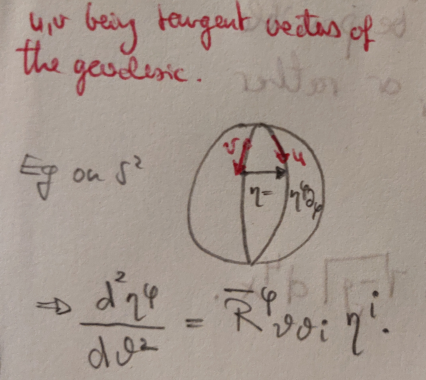
\includegraphics[width=0.7 \textwidth]{gfx/Geodesicdeviation.png}
\end{figure}
\begin{equation}
	\frac{\md ^2 \eta^{\varphi}}{\md \vartheta^2} = \bar{R}^{\varphi}_{\vartheta \vartheta i} \eta^i.
\end{equation}




\subsection{Equivalent treatment of Geodesic deviation - Caroll}
The defining property of Euclidean (flat) geometry is the parallel postulate: initially parallel lines remain
parallel forever. Of course in a curved space this is not true; on a sphere, certainly, initially
parallel geodesics will eventually cross. We would like to quantify this behavior for an
arbitrary curved space. The problem is that the notion of “parallel” does not extend naturally from flat to curved
spaces.\\
\\
Instead what we will do is to construct a one-parameter family of geodesics, $γ_s (t)$.
That is, for each $s \in \mR, γ$ is a geodesic parametrized by the affine parameter $t$. The
collection of these curves defines a smooth two-dimensional surface (embedded in a manifold
$M$ of arbitrary dimensionality). The coordinates on this surface may be chosen to be $s$ and
$t$, provided we have chosen a family of geodesics which do not cross. The entire surface is
the set of points $x^μ (s, t) \in M$. We have two natural vector fields: the tangent vectors to the
geodesics
\begin{equation}
T^\mu = \frac{\partial x^\mu}{\partial t},
\end{equation}
and the deviation vectors
\begin{equation}
S^\mu = \frac{\partial x^\mu}{\partial s}.
\end{equation}
This name derives from the informal notion that $S^μ$ points from one geodesic towards the
neighbouring ones.\\
The idea that $S^\mu$ points from one geodesic to the next inspires us to define the “relative
velocity of geodesics,”
\begin{equation}
V^\mu = (\nabla_T S)^\mu = T^\rho \nabla_\rho S^\mu
\end{equation}
and the “relative acceleration of geodesics,”
\begin{equation}
a^\mu =  (\nabla_T V)^\mu = T^\rho \nabla_\rho V^\mu.
\end{equation}
You should take the names with a grain of salt, but these vectors are certainly well-defined.\\
One finds
\begin{mybox}{Equation of geodesic deviation}
	\begin{equation}
	a^\mu = \nabla^2_{\dot{\gamma}(t)} S^\mu= \bar{R}^\mu_{\rho \sigma \nu} T^\nu T^\rho S^\sigma
	\end{equation}
	It expresses something that we might have
	expected: the relative acceleration between two neighbouring geodesics is proportional to the
	curvature.
	Physically, of course, the acceleration of neighbouring geodesics is interpreted as a manifestation of gravitational tidal forces..
\end{mybox}
















\newpage
\section{Einstein's field equations}
The field equations for gravitation are inevitably going to be more complicated than those for electromagnetism. Maxwell's equations are linear because the electromagnetic field does not itself carry charge, whereas gravitational fields do carry energy and momentum and must therefore contribute to their own source. Thus, the gravitational field equations will have to be non-linear partial differential equations, the non-linearity representing the effect of gravitation on itself.
\subsection{A not successful attempt via Poisson's equation}
Poisson’s equation can be made relativistically invariant by substituting it by
\begin{equation}
\label{eq:failedattemptEinstein}
	c^{-2} \square  \Phi = 4 \pi \mG T^\mu_\mu.
\end{equation}
In the limit of weak fields and
non-relativistic matter, this reduces to Poisson’s equation
\begin{equation}
	\Delta \Phi = 4 \pi \mG \rho.
\end{equation}
since then the time derivative in d’Alembert’s operator and the pressure contributions to T can
be neglected.\\
Why is this a problematic approach ?\\
First, the equivalence principle implies a gravitational redshift, which has been demonstrated
experimentally. One must thus require from a theory of gravity that it does lead to gravitational
redshift. However, in a theory with a Minkowskian metric, the emitted photons in an elevator,
which is at rest in a gravitational field, will propagate to the receiver at the ceiling along world
lines which may be curved, but must be parallel because the metric is constant. Hence there
cannot be gravitational redshift in a theory of gravity in flat space-time.
Second, \ref{eq:failedattemptEinstein} is a linear equation. However, there is also energy contained in the gravitational
field, which should be a source for gravity itself. So the gravitational theory cannot be linear.
Third, the gravitational potential of the Sun should be static so that the time derivative in
d’Alembert’s operator vanishes. This yields an equation which is almost identical to Poisson’s
equation except for the extra pressure contribution due to the trace of the energy-momentum
tensor on the right-hand side. Clearly, this does not give rise to a perihelion shift, which is
observed for Mercury so that the theory contradicts observations.
\\
\\
Starting off with a scalar theory of gravity, ie. one starts with the Lagrangian of a free particle in Special Relativity and multiplies it with the
factor $1 + \phi/c^2$ since this is the only possible Lagrangian that yields the right weak-field (Newtonian)
limit, one finds a perihelion shift a sixth of the actual value and with wrong sign.










\subsection{Heuristic Derivation}
In dealing with these non-linear effect we are guided once again by the Principle of Equivalence. At any point $X$ in an arbitrarily strong gravitational field, we can define a locally inertial coordinate system such that
\begin{equation}
	g\munu(X) = \eta\munu, \qquad \left(\frac{\partial g\munu(X)}{\partial x^\gamma}\right)_{x=X} =0.
\end{equation}
Hence for $x$ near $X$, the metric tensor $g\munu$ can differ from $\eta\munu$ only by terms quadratic in $x-X$. In this coordinate system the gravitational field is weak near $X$, and we can hope to describe the field by \emph{linear} partial differential equations. And once we know what these weak-field equations are, we can find the general field equations by reversing the coordinate transformation that made the field weak.\\
In the weak field limit, we have $\rho \approx T_{00}, g_{00} \approx -(1+2 \phi)$, such that the Poisson equation becomes
\begin{equation}
	\nabla^2 g_{00} = - 8 \pi \mG T_{00}.
\end{equation}
This field equation is only supposed to hold for weak static fields generated by nonrelativistic matter, and is not even Lorentz invariant as it stands. However, we can then guess 
\begin{equation}
	G_{\alpha \beta} = - 8 \pi \mG T_{\alpha \beta},
\end{equation}
where $G_{\alpha \beta}$ is a linear combination of the metric and its first and second derivatives. It follows from the principle of equivalence that the equations which govern gravitational fields of arbitrary strength must take the form
\begin{equation}
	G\munu = - 8 \pi \mG T\munu
\end{equation}
where $G\munu$ is a tensor which reduces to $G_{\alpha \beta}$ for weak fields. One can form a variety of tensors $G\munu$. In order to remove the ambiguity, we shall assume that the \emph{gravitational field equations are uniform in scale}, such that only the tensor containing $2$ derivative metric components are allowed, since the whole of $G\munu$ must have the dimensions of a second derivative. Combining all constrains one has on $G\munu$ (symmetry by symmetry of $T\munu$, conservation by conservation of $T\munu$, tensor, contains $2$ derivatives of the metric, weak field limit, Bianchi identity), one finds
\begin{equation}
	G\munu = R\munu -\half \mathcal{R}g\munu.
\end{equation}\\
\\
Without looking at failed attempts with only including $R_{\mu \nu}$ and $\nabla^2 g = 0$, one therefore finds:
\begin{equation}
	G_{\mu \nu} = \kappa T_{\mu \nu}.
\end{equation}
This equation satisfies all of the obvious requirements;
the right-hand side is a covariant expression, as required by general covariance, of the energy and momentum density in the form of a symmetric and conserved $(0, 2)$ tensor, as required by energy-momentum conservation, while the left-hand side is a symmetric and
conserved $(0, 2)$ tensor constructed from the metric, which replaces the gravitational potential, and its first and second derivatives. It
only remains to see whether it actually reproduces gravity as we know it.
With the normalization fixed by comparison
with the Newtonian limit, we can present Einstein’s equations for general relativity:
\begin{equation}
	R_{\mu \nu} - \frac{\mathcal{R}}{2} g_{ \mu \nu } = \frac{8 \pi \mathcal{G}}{c^4} T_{\mu \nu}.
\end{equation}
\marginpar{10 $2^{nd}$ order coupled, non-linear (since $G=G[g]$ and $T=T[g]$), partial differential equations for the metric.}
\begin{mybox}{Einstein's field equations}
	By heuristic derivation with $\Lambda=0$,
	\begin{equation}
	\label{eq:einsteinfieldeqs}
	G_{\mu \nu}=\frac{8 \pi \mathcal{G}}{c^4} T_{\mu \nu} \quad \Leftrightarrow \quad R_{\mu \nu}=\frac{8 \pi \mathcal{G}}{c^4} \left(T_{\mu \nu}-\frac{1}{2} g_{\mu \nu} \mathrm{Tr}T\right).
	\end{equation}
	Einstein's field equations are \emph{unique} as stated by Lovelock, i.e. $G$ must be of the form $G=\kappa T+\Lambda g$, with $\kappa$ and $\Lambda$ constants. The correct Newtonian limit then requires $\kappa = \frac{8 \pi \mathcal{G}}{c^4}$, and $\Lambda$ is the "cosmological constant".
	
\end{mybox}

In a vacuum $T\munu$ vanishes, such that the Einstein field equations in empty space are
\begin{equation}
	R\munu=0.
\end{equation}
In a space-time of two or three dimensions this would imply the vanishing of the full Riemann tensor $\bar{R}_{\mu \nu \lambda  \sigma}$, and the consequent absence of gravitational fields. It is only in four or more dimensions that true gravitational fields can exist in empty space.\\
\\
Note that in Steven Weinberg's Gravitation and Cosmology there is an alternative derivation of the Einstein field equations which is more general but very technical. It yields the insight that if we want a more general equation than Einstein's, which reduces in the weak-field limit to a second-order equation with $G_{\alpha \beta}$ on the LHS, then we must pay the price of allowing new elements unrelated to the metric tensor or its derivatives to enter, \emph{and} we must give up the possibility of deriving Newton's theory as a limiting case.
\subsubsection{On the uniqueness of Einstein's field equations via Lovelock}
Assuming that the gravitational field equations can be written in the form $D[g] = T$ , where $D[g]$
is a functional of the metric tensor $g$ and $T$ is the energy-momentum tensor, Lovelock’s theorem
states that $D[g]$ must be a linear combination of the Einstein and metric tensors, $D[g] = αG + βg$
if $D[g]$ depends on $g$ and its derivatives only up to second order. Thus, the field equations must
be of the form $G + βα^{ −1} g = α^{ −1} T$ or $G + Λg = κT$ . The correct Newtonian limit then requires
that $κ = 8π\mG c^{−4}$ , and $Λ$ is the cosmological constant.





\subsection{On the Meaning of the Field Equations}
These tell us how the curvature of spacetime reacts to the presence of energy-momentum.
Einstein’s equations may be thought of as second-order differential equations for the
metric tensor field $g_{μν}$ . There are ten independent equations (since both sides are symmetric
two-index tensors), which seems to be exactly right for the ten unknown functions of the
metric components. However, the Bianchi identity $∇_μ G^{μν} = 0$ represents four constraints on
the functions $R_{μν}$ , so there are only six truly independent equations in \ref{eq:einsteinfieldeqs}. In fact this is
appropriate, since if a metric is a solution to Einstein’s equation in one coordinate system $x^\mu$ it should also be a solution in any other coordinate system $x^{\mu^\prime}$. This means that there are
four unphysical degrees of freedom in $g_{μν}$ (represented by the four functions $x^{μ^\prime} (x^μ )$), and
we should expect that Einstein’s equations only constrain the six coordinate-independent
degrees of freedom.\\
\\
As differential equations, these are extremely complicated; the Ricci scalar and tensor are
contractions of the Riemann tensor, which involves derivatives and products of the Christoffel
symbols, which in turn involve the inverse metric and derivatives of the metric. Furthermore,
the energy-momentum tensor $T_{μν}$ will generally involve the metric as well. The equations
are also nonlinear, so that two known solutions cannot be superposed to find a third. It
is therefore very difficult to solve Einstein’s equations in any sort of generality, and it is
usually necessary to make some simplifying assumptions. Even in vacuum, where we set the
energy-momentum tensor to zero, the resulting equations
\begin{equation}
	R_{\mu \nu} = 0
\end{equation}
can be very difficult to solve. The most popular sort of simplifying assumption is that the
metric has a significant degree of symmetry, and we will talk later on about how symmetries
of the metric make life easier.
\\
\\
The nonlinearity of general relativity is worth remarking on. In Newtonian gravity the
potential due to two point masses is simply the sum of the potentials for each mass, but clearly this does not carry over to general relativity (outside the weak-field limit). There is
a physical reason for this, namely that in GR the gravitational field couples to itself. This
can be thought of as a consequence of the equivalence principle — if gravitation did not
couple to itself, a “gravitational atom” (two particles bound by their mutual gravitational
attraction) would have a different inertial mass (due to the negative binding energy) than
gravitational mass.
From a particle physics point of view this can be expressed in terms of
Feynman diagrams. The electromagnetic interaction between two electrons can be thought
of as due to exchange of a virtual photon:

\begin{figure}[h!]
	\centering
	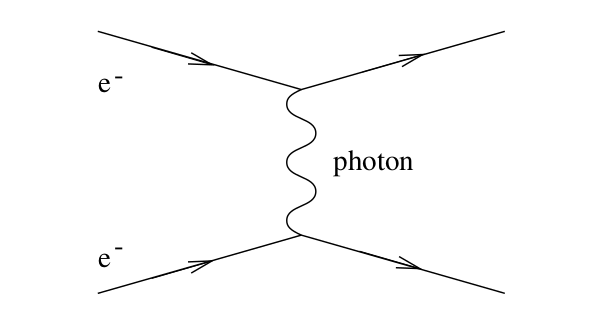
\includegraphics[width=0.7\linewidth]{gfx/QEDDiagram}
	\caption{}
	\label{fig:qeddiagram}
\end{figure}
But there is no diagram in which two photons exchange another photon between themselves;
electromagnetism is linear. The gravitational interaction, meanwhile, can be thought of
as due to exchange of a virtual graviton (a quantized perturbation of the metric). The
nonlinearity manifests itself as the fact that both electrons and gravitons (and anything
else) can exchange virtual gravitons, and therefore exert a gravitational force:

\begin{figure}[h!]
	\centering
	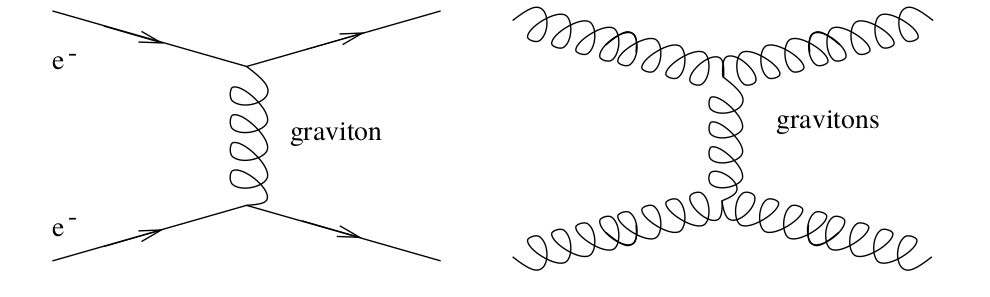
\includegraphics[width=0.7\linewidth]{gfx/GravityDiagram}
	\caption{}
	\label{fig:gravitydiagram}
\end{figure}

There is nothing profound about this feature of gravity; it is shared by most gauge theories,
such as quantum chromodynamics, the theory of the strong interactions. (Electromagnetism
is actually the exception; the linearity can be traced to the fact that the relevant gauge group,
$U(1)$, is abelian.) But it does represent a departure from the Newtonian theory.




































\newpage
\section{On the action principle - Weinberg}
There are a great many physical systems whose dynamic equations can be derived from a "principle of least action," that is, from a statement that some functional of the dynamical variables, the "action," is stationary w.r.t. small variations of these variables. This formulation of the dynamic equations has one great advantage: \emph{It allows us to establish an immediate connection between symmetry principles and conservation laws.}\\
The symmetry of the action that concerns us most in GR is general covariance. In the following, we shall develop a general definition of the energy-momentum tensor for any material system, as a functional derivative of the action for that system. The use of the action principle and general covariance will then allows us to show that this tensor is indeed conserved.\\
To achieve a truly general formulation of Gr i.t.o. an action principle, it is necessary to uncover a question that has been carefully buried until now: How can we incorporate the effects of gravitation into the field theories of particles with half-integer spin= The answer requires the tetrad formalism, which is based directly on the families of locally inertial frames.
\subsection{General definition of the Energy-Momentum-tensor by Weinberg}
We are going to define the energy-momentum tensor for a material system described by an action $S_M$ as the "functional derivative" of $S_M$ w.r.t. $g\munu$. That is, we imagine $g\munu(x)$ to be subject to an infinitesimal variation
\begin{equation}
	g\munu \rightarrow g\munu +  \delta g\munu
\end{equation}
where $\delta g\munu$ is arbitrary, except that it is required to vanish as $\abs{x^\lambda}\rightarrow\infty$. The action $S_M$ will not be stationary w.r.t. this variation, because for the moment we are regarding $g\munu(x)$ not as a dynamical variable like $x^\mu_n$ or $A_\mu$ but as an external field. Rather, $\delta S_M$ will be some linear functional of the infinitesimal $\delta g\munu(x)$, and therefore takes the form
\begin{mybox}{General definition of the energy-momentum tensor}
\begin{equation}
\label{eq:EnergyMomentumTensorWeinberg}
	\delta S_M = \half \int \md^4 x \sqrt{g(x)} T^{\mu \nu} (x) \delta g\munu(x).
\end{equation}
The coefficient $T^{\mu \nu}(x)$ is \textbf{defined} to be the energy-momentum tensor of this system. There exists a general proof that this $T^{\mu \nu}$ is a conserved symmetric tensor. 
\end{mybox}
This definition is closely analogous to a similar definition of the electric current $J^\mu$. We can break up the total matter action into a purely electromagnetic term $S_E$ and another term $S^\prime_M$ that describes the charged particles and their electromagnetic interactions
\begin{equation}
	S_M\equiv S_E+S^\prime_M \quad S_E \equiv -\frac{1}{4} \int \md^4 x \sqrt{g(x)} F\munu(x) F^{\mu \nu}(x).
\end{equation}
Consider the effect on $S^\prime_M$ of an infinitesimal variation in the vector potential $A_\mu \rightarrow A_\mu + \delta A_\mu$.
Since $S^\prime_M$ is not the whole action, the change in $S_M$ due to this variation in $A_\mu$ does not vanish, but it is necessarily a linear functional of $\delta A_\mu$:
\begin{mybox}{Definition of electromagnetic current}
	\begin{equation}
	\label{eq:electromagneticcurrent}
		\delta S^\prime_M = \int \md^4 x \sqrt{g(x)} J^\mu(x) \delta A_\mu(x)
	\end{equation}
	and the coefficient $J^\mu(x)$ is \textbf{defined} to be the electromagnetic current of the system.
\end{mybox}
\subsection{General Covariance and Energy-Momentum Conservation - Weinberg}
If the action $S_M$ for a material system is a scalar, then the statement that $\delta S_M$ vanishes is generally covariant, and also are the dynamical equations derived from this statement.\\
We shall therefore assume that $S_M$ is a scalar. This means that $S_M$ will be unchanged if we replace $x^\mu_n, A_\mu,g\munu$ by their primed values. If the original transformation $x^\mu\rightarrow x^{\prime \mu} $ was infinitesimal:
\begin{equation}
	x^{\prime \mu} = x^\mu + \epsilon^\mu(x)
\end{equation}
then the change in the dynamical variables is a change in 
\begin{align}
	\label{eq:variationalprincipleVariableChange}
\delta x^\mu_n(p) &= \epsilon^\mu(x_n(p)) \\
\delta A_\mu(x) &= -A_\nu(x) \frac{\partial \epsilon^\nu (x)}{\partial x^\mu} - \frac{\partial A_\mu(x)}{\partial x^\nu} \epsilon^\nu(x)\\
\delta g\munu(x) &= -g_{\mu \lambda} (x) \frac{\partial \epsilon^\lambda(x)}{\partial x^\nu} - g_{\lambda \nu} (x) \frac{\partial \epsilon^\lambda}{\partial x^\mu} - \frac{\partial g\munu(x)}{\partial x^\lambda} \epsilon^\lambda(x).
\end{align} 
The important point is that this is now an infinitesimal transformation of the dynamical variables alone, not of the coordinates over which we integrate, so the principle of stationary actions tells us that when the dynamical equations for $x^\mu_n$, $A_\mu$, and so on, are satisfied the change in these quantities produces no change in the matter action $S_M$. The only changes in $S_M$ comes from the variation in the external field $g\munu$, and \ref{eq:EnergyMomentumTensorWeinberg} gives for this change
\begin{equation}
	\delta S_M = - \half \int \md^4 x \sqrt{g} T^{\mu \nu} \left[g_{\mu \lambda} \frac{\partial \epsilon^\lambda}{\partial x^\nu} + g_{\lambda \nu} \frac{\partial \epsilon^\lambda}{\partial x^\mu} + \frac{\partial g\munu}{\partial x^\lambda} \epsilon^\lambda\right].
\end{equation}
If $S_M$ is a scalar, then this must vanish; integrating by parts gives then
\begin{equation}
	0 = \delta S_M=\int \md^4 x \epsilon^\lambda \left[ \frac{\partial}{\partial x^\nu} \left(\sqrt{g} T^\nu_\lambda\right)-\half \left(\frac{\partial g\munu}{\partial x^\lambda}\right)\sqrt{g} T^{\mu \nu}\right]
\end{equation}
and since $\epsilon^\lambda$ is arbitrary
\begin{equation}
	0 = \frac{\partial}{\partial x^\nu} \left(\sqrt{g} T^\nu_\lambda\right) - \half \left(\frac{\partial g\munu}{\partial x^\lambda}\right) \sqrt{g} T^{\mu \nu}
\end{equation}
or equivalently
\begin{mybox}{General Covariance implies Energy-momentum Conservation}
	\begin{equation}
		0= (T^\nu_\lambda)_{;\nu}.
	\end{equation}
	\textbf{Thus the energy-momentum tensor defined by Eq. \ref{eq:EnergyMomentumTensorWeinberg} is conserved (in the covariant sense) if and only if the matter action is a scalar}. Also, with $S_M$ a scalar, \ref{eq:EnergyMomentumTensorWeinberg} shows immediately that $T^{\mu \nu}$ is a symmetric \textbf{tensor}, so this definition of the energy-momentum tensor has all the properties for which one could wish.\\
	\textbf{This proof, that general covariance implies energy-momentum conservation, has an exact analogue in the proof that gauge invariance implies charge conservation}
\end{mybox}
The change in $S^\prime_M$ caused by an arbitrary gauge transformation can arise only form the change in $A_\mu$, since $S^\prime_M$ is stationary w.r.t. all other dynamical variables. A general infinitesimal gauge transformation $\epsilon$ will produce in $A_\mu$ the change $\delta A_\mu = \frac{\partial \epsilon}{\partial x^\mu}$. Inserting this in \ref{eq:electromagneticcurrent}, we see that $S^\prime_M$ is gauge invariant if and only if
\begin{equation}
0 = \delta S^\prime_M = \int \md^4 x \sqrt{g}J^\mu \frac{\partial \epsilon}{\partial x^\mu}.
\end{equation}
Integrating by parts gives
\begin{equation}
	0=\int \md^4 x \epsilon \frac{\partial}{\partial x^\mu} \left(\sqrt{g} J^\mu\right)
\end{equation}
or, since $\epsilon$ is arbitrary
\begin{equation}
	0=\frac{1}{\sqrt{g}} \frac{\partial}{\partial x^\mu} \sqrt{g} J^\mu = J^\mu_{;\mu},
\end{equation}
implying charge conservation. \\
\emph{We see again how closely analogous are gauge invariance and general covariance.}
\subsubsection{Applications of the general energy momentum tensor: Einstein's field equations and Contracted Bianchi identity}
So far, the gravitational field $g\munu$ has been an external field that could be prescribed at will . (Indeed, \ref{eq:EnergyMomentumTensorWeinberg} usually provides the most convenient definition of the energy-momentum tensor even in the absence of gravitation.) We will now give $g\munu$ equations of its own, by adding to the total action $S$ a purely gravitational term $S_G$:
\begin{equation}
	S=S_M+S_G,
\end{equation}
\begin{equation}
	S_G \equiv - \frac{1}{16 \pi \mG} \int \sqrt{g(x)} \mathcal{R}(x) \md^4 x.
\end{equation}
Clearly $S_G$ is a scalar, so this would be a good candidate for a theory of gravitation even if we had no experience with gravitational phenomena. The application to $S$ of the principle of stationary action does in fact yields the Einstein field equations. This is further explored below.\\
Another application of \ref{eq:EnergyMomentumTensorWeinberg} besides the derivation of the Einstein field equations is to use it to derive the contracted Bianchi identity. Since $S_G$ is a scalar it must be stationary wr.t. variation \ref{eq:variationalprincipleVariableChange} in $g\munu$. Repeating the reasoning that led before to general covariance implying energy-momentum conservation, we now find that
\begin{equation}
	\left[R^\nu_\lambda - \half \delta^\nu_\lambda \mathcal{R}\right]_{;\nu} = 0
\end{equation}
which we recognize as the contracted Bianchi identity.\\
This formalism suggests that Einstein's theory might be modified by adding to $\mathcal{R}$ in the Einstein-Hilbert action terms proportional to $\mathcal{R}^2,\mathcal{R}^3,\dots$. Such terms would only show up on a sufficiently small space-time scale.
















\newpage
\section{Derivation of Einstein's Field Equations from Least Action Principle}
\marginpar{Lorentz-covariance $\Rightarrow$ scalar $\Rightarrow$ $\mathcal{R}$. All $\mathcal{R}^n$ are allowed, but $n=1$ is the simplest.}
\marginpar{Introduce normal coordinates where $\Gamma=0$, then arrive at tensor equality ($\partial \rightarrow \nabla$) to have generality of frame again.}

Since we only apply the Principle of General Covariance on a small scale compared with the scale of the gravitational field, we usually expect that it is only $g\munu$ and its first derivatives that enter our generally covariant equations. \emph{This is precisely what we need to construct the Einstein-Hilbert action solely from the Ricci scalar, thus assume Principle of General Covariance and we can then postulate that the invariant scalar of the theory should only depend on the metric and its first derivatives.}
The Lagrange density is a tensor density, which can be written as $\sqrt{−g }$ times a scalar. What
scalars can we make out of the metric? Since we know that the metric can be set equal to
its canonical form and its first derivatives set to zero at any one point, any non-trivial scalar
must involve at least second derivatives of the metric. The Riemann tensor is of course
made from second derivatives of the metric, and we argued earlier that the only independent
scalar we could construct from the Riemann tensor was the Ricci scalar $\mathcal{R}$. What we did not
show, but is nevertheless true, is that any non-trivial tensor made from the metric and its
first and second derivatives can be expressed in terms of the metric and the Riemann tensor.
Therefore, the only independent scalar constructed from the metric, which is no higher than
second order in its derivatives, is the Ricci scalar. Hilbert figured that this was therefore the
simplest possible choice for a Lagrangian, and proposed
\begin{equation}
	S_{\mathrm{EH}} [g] = \int_{D\subset M} \mathcal{R}[g] \eta = \int_D \mathcal{R}[g] \sqrt{-g} \md^4 x.
\end{equation}
To repeat, the reasoning is:\\
What we want for the construction of our theory is not a tensor, but a completely invariant thing to put into the Lagrangian. (Instead, Einstein said that the Stress-Energy Tensor equals another tensor, which is derivable from the curvature tensor.) The least-action principle must involve an integral over all space, which must be completely invariant to transformations. The integrand must be a world scalar:
\begin{equation}
\int \md^4 x (Scalar) = (Scalar \, invariant).
\end{equation}
We get such a scalar via the Ricci scalar. Now, the volume integral of this scalar is not invariant, because the volume element is not a scalar, need to use canonical volume form thus to altogether arrive at the Einstein-Hilbert action for empty space. The remarkable uniqueness of $\mathcal{D}[g]$ shown by Lovelock indicates that a Lagrangian formulation of GR should be possible starting from a scalar constructed from $\mathcal{D}$, or rather $\mathrm{Tr}\mathcal{D} \propto \mathcal{R}$.\\\\
\\
The equations of motion should come from varying the action with respect to the metric. The fact that gravity is attractive for likes and unlikes is a property of the Lagrangian, so that if we change $S\rightarrow -S$, the force changes sign. Note that the sign of the coupling constant $e,g,\lambda$ makes no difference, since it appears as a square in any diagram which represents a correction to the energy. The sign of the Coulomb forces comes from the sign of the time components in the Lagrangian. For gravity waves, since we are contracting over two indices, the signs cancel out and we have attraction. In fact let us consider variations with respect to the inverse metric $g^{\mu \nu}$ , which are slightly
easier but give an equivalent set of equations. Using $\mathcal{R} = g^{μν} R_{μν}$ , in general we will have
\begin{align}
	\delta S &=  \int \md^n x \left[\sqrt{-g} g^{\mu \nu} \delta R_{\mu \nu} + \sqrt{-g} R_{\mu \nu} \delta g^{\mu \nu} + \mathcal{R} \delta \sqrt{-g})\right] \\
	&= (\delta S)_1 + (\delta S)_2 + (\delta S)_3 \nonumber.
\end{align}
The second term $(δS)_2$ is already in the form of some expression times $δg^{μν}$ ; let’s examine
the others more closely.\\
Recall that the Ricci tensor is the contraction of the Riemann tensor, which is given by
\begin{equation}
	R^\rho_{\mu \lambda \nu} = \partial_\lambda \Gamma^\lambda_{\nu \mu} + \Gamma^\rho_{\lambda \sigma}\Gamma^\sigma_{\nu\mu} - (\lambda \leftrightarrow \nu). 
\end{equation}
The variation of this with respect the metric can be found first varying the connection with
respect to the metric, and then substituting into this expression. Let us however consider arbitrary variations of the connection, by replacing
\begin{equation}
	\Gamma^\rho_{\mu \nu} \rightarrow\quad \Gamma^\rho_{\mu \nu} + \delta \Gamma^\rho_{\mu \nu}.
\end{equation}
The variation $δΓ^ρ_{νμ}$ is the difference of two connections, and therefore is itself a tensor. We
can thus take its covariant derivative,
\begin{equation}
∇_λ (δΓ^ρ{νμ} ) = ∂_λ (δΓ^\rho_{\nu μ} ) + Γ^ρ_{λσ} δΓ^σ_{νμ} − Γ^σ_{λν} δΓ^ρ_{σμ} − Γ^σ_{λμ} δΓ^ρ_{νσ} .
\end{equation}
Given this expression it is easy to show that
\begin{equation}
	δR^ρ_{μλν} = ∇_λ (δΓ^ρ_{νμ} ) − ∇_ν (δΓ^ρ_{λμ} ).
\end{equation}
Therefore
\begin{align}
	(\delta S)_1 &= \int \md^n x \sqrt{−g} g^{μν} \left[ ∇_λ (δΓ^λ_{νμ} ) − ∇_ν (δΓ^λ_{λμ} )	\right]		 \nonumber \\
	&= \int \md^n x \sqrt{−g} ∇_σ \left[g^{μσ} (δΓ^λ_{λμ} ) − g^{μν} (δΓ^σ_{μν} ) \right],
\end{align}
where we have used metric compatibility and relabelled some dummy indices. But now we
have the integral with respect to the natural volume element of the covariant divergence of
a vector; by Stokes’s theorem, this is equal to a boundary contribution at infinity which we
can set to zero by making the variation vanish at infinity. Therefore this term contributes nothing
to the total variation.\\
To make sense of the $(δS)_3$ term we need to use the following fact, true for any matrix
$M$:
\begin{equation}
	\tr(\ln(M)) = \ln(\det M).
\end{equation}
Here, $\ln M$ is defined by $\exp(\ln M) = M$. The variation of this identity yields
\begin{equation}
	\tr(M^{-1} \delta M) = \frac{1}{\det(M)} \delta\left(\det(M)\right).
\end{equation}
Here we have used the cyclic property of the trace to allow us to ignore the fact that $M^{−1}$
and $δM$ may not commute. Now we would like to apply this to the inverse metric, $M = g^{μν}$. Then $\det M = g^{−1}$ (where $g = \det g_{μν}$ ), and
\begin{equation}
	\delta(g^{-1}) = \frac{1}{g} g_{\mu \nu}\delta g^{\mu \nu}.
\end{equation}
Now we can just plug in
\begin{align*}
	\delta \sqrt{-g} &= \delta \left[(-g^{-1})^{-\half}\right] \\
	&=- \half ((-g^{-1})^{-3/2} ) \delta(- g^{-1})\\
	&= -\half \sqrt{-g} g_{\mu \nu} \delta g^{\mu \nu}.
\end{align*}
Altogether, we thus find
\begin{equation}
	\delta S = \int \md^n x \sqrt{-g}  \left[R_{\mu \nu} - \frac{\mathcal{R}}{2} g_{\mu \nu} \right]\delta g^{\mu \nu}.
\end{equation}
This should vanish for arbitrary variations, so we are led to Einstein’s equations in vacuum:
\begin{equation}
	\frac{1}{\sqrt{-g}} \frac{\delta S}{\delta g^{\mu \nu}} = G_{\mu \nu} =0.
\end{equation}
What we would really like, however, is to get the non-vacuum field equations
as well. That means we consider an action of the form
\begin{equation}
	S = \frac{c^4}{8 \pi \mathcal{G}} S_{EH} + S_M
\end{equation}
where $S_M$ is the action for matter, and we have presciently normalized the gravitational
action. Following through the same procedure as above yields:
\begin{equation}
		\frac{1}{\sqrt{-g}} \frac{\delta S}{\delta g^{\mu \nu}} = \frac{c^4}{8 \pi \mathcal{G}} G_{\mu \nu} + \frac{1}{\sqrt{-g}} \frac{\delta S_M}{\delta g^{\mu \nu}},
\end{equation}
and we recover Einstein’s equations if we can set
\begin{equation}
\label{eq:GRenergymomentumtensor}
	T_{\mu \nu} = - \frac{2}{\sqrt{-g}} \frac{\delta S_M}{\delta g^{\mu \nu}}.
\end{equation}
What makes us think that we can make such an identification? In fact \ref{eq:GRenergymomentumtensor} turns out to
be the best way to define a symmetric energy-momentum tensor. The tricky part is to show
that it is conserved, which is in fact automatically true, but which we will not justify until
the next section.
\subsubsection{On the definition of energy-momentum tensors}
We say that \ref{eq:GRenergymomentumtensor} provides the “best” definition of the energy-momentum tensor because
it is not the only one you will find. In flat Minkowski space, there is an alternative definition which is sometimes given in books on electromagnetism or field theory. In this context energy-momentum conservation arises as a consequence of symmetry of the Lagrangian under spacetime translations. Noether’s theorem states that every symmetry of a Lagrangian
implies the existence of a conservation law; invariance under the four spacetime translations
leads to a tensor $S_{μν}$ which obeys $∂^\mu S_{μν} = 0$ (four relations, one for each value of $ν$). Applying Noether’s
procedure to a Lagrangian which depends on some fields $ψ^i$ and their first derivatives $∂_μ ψ^i$ ,
we obtain
\begin{equation}
\label{eq:canonicalenergymomentumtensor}
	S_{μν} =\sum_i \frac{\delta \mL}{\delta (\partial_\mu \psi^i)} ∂_ν ψ^i − η_{μν} \mL.
\end{equation}
You can check that this tensor is conserved by virtue of the
equations of motion of the matter fields. $S_{μν}$ often goes by the name “\emph{canonical energy-momentum tensor}”; however, there are a number of reasons why it is more convenient for
us to use \ref{eq:GRenergymomentumtensor}.
\begin{enumerate}
	\item \ref{eq:GRenergymomentumtensor} is in fact what appears on the right hand side of
	Einstein’s equations when they are derived from an action, and it is not always possible to
	generalize \ref{eq:canonicalenergymomentumtensor} to curved spacetime.
	\item But even in flat space \ref{eq:GRenergymomentumtensor} has its advantages; it is
	manifestly symmetric, and also guaranteed to be gauge invariant, neither of which is true for
	\ref{eq:canonicalenergymomentumtensor}.\\
	Since the Lagrangian changes if the gauge is changed, the canonical energy-momentum tensor (from SR) is not gauge invariant. This is a reflection of the non-localizability of the gravitational energy. Even in the linearised theory, it is not possible to find gauge invariant expressions for the energy and momentum densities.
\end{enumerate}
Note also that the canonical energy momentum tensor can be viewed as a generalization of the prescription to obtain the Hamiltonian, i.e. the energy, of a system from the corresponding Lagrangian via a Legendre transformation. Note further that the canonical energy-momentum tensor is not generally symmetric, the resulting theory is pathological ( there is no way to define angular momentum in the field for example). One can in fact add the Belinfante-Rosenfeld tensor to the canonical energy-momentum tensor in order to obtain a symmetric and conserved energy momentum tensor. Thus we see that corrections to the canonical Noether tensor that appear in the Belinfante-Rosenfeld tensor occur because we need to simultaneously vary the vierbein and the spin connection if we are to preserve local Lorentz invariance, c.f. BR tensor on Wikipedia.
\begin{mybox}{Weak Energy condition}
	Our real concern is with the
	existence of solutions to Einstein’s equations in the presence of “realistic” sources of energy
	and momentum, whatever that means. The most common property that is demanded of
	$T_{μν}$ is that it represent positive energy densities — no negative masses are allowed. In a
	locally inertial frame this requirement can be stated as $ρ = T_{00} ≥ 0$. To turn this into a coordinate-independent statement, we ask that
	\begin{equation}
	T_{\mu \nu} V^{\mu} V^{\nu} \geq 0 \quad \forall \; \mathrm{time-like} \; V^\mu
	\end{equation}
	This is known as the \emph{Weak Energy Condition}, or WEC.
\end{mybox}
Unfortunately it is not set in stone; indeed, it is straightforward to invent
otherwise respectable classical field theories which violate the WEC, and almost impossible
to invent a quantum field theory which obeys it. Nevertheless, it is legitimate to assume
that the WEC holds in all but the most extreme conditions.

\subsubsection{The trace of the energy-momentum tensor}
Consider a conformal transformation of the metric
\begin{equation}
	g^{\mu \nu}(x) \rightarrow e^{\lambda(x)} g^{\mu \nu}(x) \approx g^{\mu \nu} + \underbrace{\delta g^{\mu \nu}}_{\lambda g^{\mu\nu}}.
\end{equation}
With the definition of the energy momentum tensor
\begin{equation}
	T\munu = -  \frac{1}{\sqrt{-g}} \frac{\delta S}{\delta g\munu}
\end{equation}
we find for the variation of the action
\begin{align}
	\delta S &= \int \md^4 x \sqrt{-g} \frac{\delta S}{\delta g_{\mu \nu}} \delta g_{\mu \nu} \\
	&= - \int \md^4 x \sqrt{-g}^2 T^{\mu \nu} \lambda g\munu \\
	&= -\int \md^4 x \sqrt{-g}^2 \lambda T^\mu_\mu \\
	T^\mu_\mu = 0 \quad &\Rightarrow \delta S =
\end{align}
under conformal transformation. Thus, if the energy-momentum tensor has a vanishing trace, then it is
scale-invariant (under conformal transformation). Therefore, the corresponding theory is scale-invariant.



\subsection{The full Einstein field equations}
We have now justified Einstein’s equations in two different ways: as the natural covariant
generalization of Poisson’s equation for the Newtonian gravitational potential, and as the
result of varying the simplest possible action we could invent for the metric.\\
\\
\begin{mybox}{Einstein's field equations including $\Lambda$}
A constant
does not by itself lead to very interesting dynamics, it has an important effect if we add it
to the conventional Hilbert action. We therefore consider an action given by
\begin{equation}
	S =  \int_D \left(\mathcal{R}+2 \Lambda\right) \eta,
\end{equation}
\emph{Einstein's vacuum equations}, 
\begin{equation}
	G - \Lambda g=0,
\end{equation}
\end{mybox}
\marginpar{Variation is performed w.r.t $g$, later also $\delta g$, since $\delta \psi$ yields \emph{matter field equations}. This is frame independent since $\delta \mathcal{J}$ as $\mathcal{J}[g] = \mathcal{J}$.}
The complete equations are obtained by coupling gravity/geometry and matter.\\
Ignored possible boundary since $\delta g$ only inside $D$, include Gibbons-Hawking-York boundary term for manifold with boundary.\\
For $\Lambda$ on the RHS, $Λ$ can be interpreted as the “energy density of the vacuum,”
a source of energy and momentum that is present even in the absence of matter fields. This
interpretation is important because quantum field theory predicts that the vacuum should
have some sort of energy and momentum. In ordinary quantum mechanics, an harmonic
oscillator with frequency $ω$ and minimum classical energy $E_0 = 0$ upon quantization has a
ground state with energy $E_0 = \half h̄ω$. A quantized field can be thought of as a collection of
an infinite number of harmonic oscillators, and each mode contributes to the ground state
energy. The result is of course infinite, and must be appropriately regularized, for example 
by introducing a cut-off at high frequencies. The final vacuum energy, which is the regularized
sum of the energies of the ground state oscillations of all the fields of the theory, has no good
reason to be zero and in fact would be expected to have a natural scale $\Lambda \propto M^4_{pl}$, here the Planck mass is approximately $10^{19} GeV$, or $10^{−5} grams$. Observations of the
universe on large scales allow us to constrain the actual value of $Λ$, which turns out to be
smaller than $M^4_{pl}$ by at least a factor of $10^{120}$ . This is the largest known discrepancy between
theoretical estimate and observational constraint in physics, and convinces many people that
the “cosmological constant problem” is one of the most important unsolved problems today.
On the other hand the observations do not tell us that $Λ$ is strictly zero, and in fact allow
values that can have important consequences for the evolution of the universe. This mistake
of Einstein’s therefore continues to bedevil both physicists, who would like to understand
why it is so small, and astronomers, who would like to determine whether it is really small
enough to be ignored.

\subsubsection{This is how we use diffeomorphism invariance to postulate Einstein-Hilbert action}
We choose the action for the gravitational field to be
\begin{equation}
S_g = -\frac{1}{2 \lambda^2} \int \md^4x \mathcal{R}\sqrt{-g}.
\end{equation}
The curvature tensor appears when we take the variation of $S_g$ w.r.t. $g\munu$
\begin{equation}
\frac{\delta S_g}{\delta g\munu} = \frac{1}{2 \lambda^2} \sqrt{-g} \left(R^{\mu \nu} - \half \mathcal{R} g^{\mu \nu}\right).
\end{equation}
It is because of this that we can use the integral of $\mathcal{R}$ as the action of the gravitational part of the complete problem.
That because this stress tensor appears in this way, from a variational principle, its covariant divergence is neccessarily zero. We have seen the connection from the other direction-that we could deduce a variational principle provided that we started from a divergenceless tensor. \\
We want to show that if the functional 
\begin{equation}
S_g = \int \md^4 x \Sigma[g\munu]
\end{equation}
is invariant under coordinate transformations, then the covariant divergence of the variation of $S_g$ w.r.t. $g\munu$ is identically zero. Under the infinitesimal transformation to primed coordinates
\begin{equation}
x^\mu = x^{\mu^\prime} + h^\mu(x^\prime),
\end{equation}
the functional changes as, dropping primes on integration variables
\begin{equation}
S_g = \int \md^4 x \Sigma[g^\prime\munu] = \int \md^4 x \Sigma[g\munu] + \int \md^4x \frac{\delta \Sigma}{\delta g\munu} (h^\alpha_{,\nu} g_{\mu \alpha} + h^\alpha_{,\mu} g_{\nu \alpha} + h^\alpha g_{\mu \nu,\alpha} ).
\end{equation}
When we do an integration by parts on the second term of this expression, we convert it to an expression involving the functional derivatives of the function $\Sigma$. We it it equal to zero, since we know that the change in the action must be zero for any $h^\alpha$, because of the character of $\Sigma$.
\begin{equation}
\label{eq:Feynman1}
\frac{\partial}{\partial x^\mu} \left[\frac{\delta \Sigma}{\delta g\munu} g_{\nu \alpha}\right] - \half \frac{\delta \Sigma}{\delta g\munu} \frac{\partial g\munu}{\partial x^\alpha} = 0.
\end{equation}
Let us denote by $\mG^{\mu \nu}$ the variation of $2 \lambda^2 S_g$ w.r.t. $g\munu$:
\begin{equation}
\mG^{\mu \nu} = 2 \lambda^2 \frac{\delta Ŝ_g}{\delta g\munu}.
\end{equation}
This quantitiy is a contravariant tensor density of second rank, thus \ref{eq:Feynman1} becomes
\begin{equation}
(g_{\alpha\mu} \mG^{\mu \nu})_{,\nu} - \half g_{\mu \nu,\alpha} \mG^{\mu \nu} =,
\end{equation}
which is equivalent to the statement that the covariant divergence of $\mG^{\mu \nu}$ iszero:
\begin{equation}
\label{eq:Feynman2}
\mG^{\mu \nu}_{;\nu} = 0.
\end{equation}
Using tensor and covariant derivative formulae as written above, it is quite straightforward to deduce that \ref{eq:Feynman1} and \ref{eq:Feynman2} are equivalent. Thus, we see that the invariance of an action results in the  construction of a \emph{tensor density} which is automatically divergenceless. The tensor associated with the tensor density $\mG^{\mu \nu}$  is also divergenceless
\begin{equation}
G^{\mu \nu} = \mG^{\mu \nu} / \sqrt{-g}, \quad G^{\mu \nu}_{;\nu} =0.
\end{equation}



\subsection{Coordinate Conditions - A note on gauge freedom in Einstein's field equations -Weinberg}
\label{subsec:gaugefreedomGR}
The symmetric tensor $G\munu$ has $10$ independent components, so Einstein's field equations comprise $10$ algebraically independent equations. The unknown metric tensor also has $10$ algebraically independent components, and at first sight one would think that Einstein equations (with appropriate boundary conditions) would suffice to determine the $g\munu$ uniquely. However, this is not so. Although algebraically independent, the $10\, G\munu$ are related by four differential identities, the Bianchi identities:
\begin{equation}
G^\mu_{\nu ; \mu} = 0,
\end{equation}
which are a \emph{reduction of equations (Gauge freedom)}. Thus there are not $10$ functionally independent equations, but only $10-4=6$, leaving us with four degrees of freedom in the $10$ unknowns $g\munu$. These degrees of freedom correspond to the fact that if $g\munu$ is a solution of Einstein's equation, then so is $g^\prime\munu$, where $g^\prime\munu$ is determined from $g\munu$ by a general coordinate transformation $x\rightarrow x^\prime$. Such a coordinate transformation involves four arbitrary functions $x^{\mu^\prime} (x)$, giving to the solutions of the field equations \ref{eq:einsteinfieldeqs} just four degrees of freedom.\\
\subsubsection{Comparison with gauge freedom in EM}
The failure of Einstein's equations to determine $g\munu$ uniquely is closely analogous with the failure of Maxwell's equations to determine the vector potential $A_\mu$ uniquely, hence these redundancies in the degrees of freedom are a \emph{gauge freedom}. When written i.t.o. the vector potential, Maxwell's equations read
\begin{equation}
\label{eq:eomVectorPotentialEM}
\square A_\alpha - \frac{\partial^2}{\partial x^\alpha \partial x^\beta} A^\beta = - J_\alpha.
\end{equation}
There are four equations for the four unknowns, but they do no determine $A_\alpha$ uniquely, because the LHS of these equations are related by a differential identity analogous to the Bianchi identity
\begin{equation}
\frac{\partial}{\partial x^\alpha} \left[\square A^\alpha - \frac{\partial^2}{\partial x_\alpha \partial x^\beta} A^\beta \right] \equiv 0.
\end{equation}
Thus the number of functionally independent equations is really only $4-1=3$, and there is one degree of freedom in the solution of the four $A_\alpha$. This degree of freedom of course corresponds to \emph{gauge invariance}; given any solution $A_\alpha$, we can find another solution $A^\prime_\alpha \equiv A_\alpha + \frac{\partial \Lambda}{\partial x^\alpha}$, with $\Lambda$ arbitrary.\\
The ambiguity in the solutions of Maxwell's and Einstein's equations can be removed by main force. In the case of Maxwell's equation we do this by choosing a particular gauge. For instance, given any solution $A_\alpha$, we can always construct a solution $A^\prime_\alpha$ such that
\begin{equation}
\label{eq:LorentzGaugeEM}
\partial_\alpha A^{\prime \alpha} =0
\end{equation} 
by setting
\begin{equation}
A^\prime_\alpha \equiv A_\alpha + \frac{\partial \Phi}{\partial x^\alpha}
\end{equation}
where $\Phi$ is defined by
\begin{equation}
\square\Phi = - \frac{\partial A^\alpha}{ \partial x^\alpha}.
\end{equation}
Such a solution is said to be in the \emph{Lorentz gauge}.\\
The condition \ref{eq:LorentzGaugeEM} when added to the \emph{three} independent equations \ref{eq:eomVectorPotentialEM} completes a system of four equations that, with appropriate boundary conditions, will generally determine the four $A_\alpha$ uniquely.
\subsubsection{Adopt the same philosophy for the gauge freedom in GR}
In the same ways, we can eliminate the ambiguity in the metric tensor by adopting some particular coordinate system(i.e. the redundancy of coordinate systems is the gauge freedom in GR). The choice of a coordinate system can be expressed in four \emph{coordinate conditions}, which, when added to the six independent Einstein equations, determine an unambiguous solution.\\
\begin{mybox}{Harmonic coordinate condition}
	One particular convenient choice of a coordinate system is represented in the \emph{harmonic coordinate conditions}
	\begin{equation}
	\label{eq:harmoniccoordinatecondition}
	\Gamma^\lambda \equiv g^{\mu \nu} \Gamma^\lambda\munu =0.
	\end{equation}
	It is always possible to choose a coordinate system in which this holds, since, if $\Gamma^\rho$ does not vanish, we can always define a new coordinate system $x^{\prime \lambda}$ by solving the second-order partial differential equations
	\begin{equation}
	g^{\rho \sigma} \frac{\partial^2 x^{\prime \lambda}}{\partial x^\rho \partial x^\sigma} = \frac{\partial x^{\prime \lambda}}{\partial x^\rho} \Gamma^\rho
	\end{equation}
	and contracting \ref{eq:christoffelTrafo} to the form $\Gamma^{\prime \lambda} =..$ then yields $\Gamma^{\prime \lambda}=0$ in the $x^\prime$-system.
\end{mybox}
The four conditions \ref{eq:harmoniccoordinatecondition} are of course not generally covariant, since their purpose is to remove the ambiguity in the metric tensor owing to the general covariance of the Einstein equations.
\begin{mybox}{Equivalent form of the harmonic coordinate condition}
	With the contracted Christoffel i.t.o. the metric tensor, one finds
	\begin{equation}
	\label{eq:harmoniccoordinateconditionEquivalent}
	\frac{\partial}{\partial x^\kappa} \left(\sqrt{g} g^{\lambda \kappa}\right)=0.
	\end{equation}
\end{mybox}
\begin{mybox}{Harmonic coordinates definition}
	We are now in a position to explain the term "harmonic coordinates". A function $\phi$ is said to be harmonic if $\square^2 \phi$ vanishes,
	where $\square^2$ is the \emph{invariant} or \emph{covariant d'Alembertian}
	\begin{equation}
	\square^2 \phi \equiv \left(g^{\lambda \kappa} \phi_{;\lambda} \right)_{;\kappa} = g^{\lambda \kappa} \frac{\partial^2 \phi}{\partial x^\lambda \partial x^\kappa} - \Gamma^\lambda \frac{\partial \phi}{\partial x^\lambda}.
	\end{equation}
\end{mybox}
\begin{mybox}{"Harmonic Gauge" - harmonic coordinate condition in $x^\mu$}
	If $\Gamma^\lambda=0$ then the coordinates are themselves harmonic functions,
	\begin{equation}
	\label{eq:harmonicCoordinatesGauge}
	\square^2 x^\mu = 0
	\end{equation}
	thus justifying our application of the adjective "harmonic" to such coordinate systems.
\end{mybox}
In the absence of gravitational fields, the obvious harmonic coordinate system is that of Minkowski, in which $g^{\lambda \kappa} = \eta^{\lambda \kappa}$ and $g=1$, so that \ref{eq:harmoniccoordinateconditionEquivalent} is satisfied trivially. In the presence of weak gravitational fields the harmonic coordinate systems may be pictured as nearly Minkowskian. Another related advantage of the harmonic coordinate condition is that, as shown later on, its use produces a very great simplification in the weak-field equations, similar to the simplification brought to Maxwell's equations by use of the Lorentz gauge, c.f. Weak field treatment in \ref{ch:GRapplications}.








\section{The energy-momentum tensor}
\subsection{Energy, Momentum, and Angular Momentum of Gravitation - Weinberg}
Similar to the linear gravity analysis in \ref{ch:GRapplications}, we adopt here a coordinate system that is quasi-Minkowskian, in the sense that the metric $g\munu$ approaches the Minkowski metric $\eta\munu$ at great distances from the finite matter system under study. (This is the case in harmonic coordinate systems, and others as well.) We then write
\begin{equation}
	g\munu = \eta\munu + h\munu
\end{equation}
so that $h\munu$ vanishes at infinity. (However, $h\munu$ is not assumed to be small everywhere.)  The part of the Ricci tensor linear in $h\munu$ is then
\begin{equation}
R^{(1)}_{\mu \kappa} \equiv \half \left[\frac{\partial^2 h^\lambda_\lambda}{\partial x^\mu \partial x^\kappa} - \frac{\partial^2 h^\lambda_\mu}{\partial x^\lambda \partial x^\kappa } - \frac{\partial^2 h^\lambda_\kappa }{\partial x^\lambda \partial x^\mu} + \frac{\partial^2 h_{\mu \kappa}}{\partial x^\lambda \partial x_\lambda}\right].
\end{equation}
We are adopting the convenient convention that indices on $h\munu, R^{(1)}\munu$, and $\partial/\partial x^\lambda$ are raised and lowered with $\eta$s, for example, $h^\lambda_\lambda \equiv \eta^{\lambda \nu} h_{\lambda \nu}$ and $\partial/\partial x_\lambda \equiv \eta^{\lambda \nu} \partial/\partial x^\nu$, whereas indices on true tensors such as $R\munu$ are raises and lowered with $g$s as usual. 
\begin{mybox}{Energy-momentum tensor of gravity}
	The exact Einstein equations linearized in the perturbation can then be written as
	\begin{equation}
	\label{eq:linearizedEinstein}
	R^{(1)}_{\mu \kappa} - \half \eta_{\mu \kappa} R^{(1)\lambda}_\lambda = - 8 \pi \mG \left[T_{\mu \kappa} + t_{\mu \kappa} \right]
	\end{equation}
	where
	\begin{equation}
		\label{eq:energymomentumtensorofGravity}
		t_{\mu \kappa} \equiv \frac{1}{8 \pi \mG} \left[R_{\mu \kappa} - \half g_{\mu \kappa} R^\lambda_\lambda - R^{(1)}_{\mu \kappa} + \half \eta_{\mu \kappa} R^{(1)\lambda}_\lambda\right].
	\end{equation}
	Equation \ref{eq:linearizedEinstein} has just the form we should expect for the wave equation of a field of spin $2$  but with the peculiarity that its "source" $T\munu+t\munu$ depends explicitly on the field $h\munu$. We interpret this feature by saying that the field $h\munu$ is generated by the total densities and fluxes of energy and momentum, and 
	\textbf{$t\munu$ is simply the energy-momentum "tensor" of the gravitational field itself}. \\
		\end{mybox}
	\begin{mybox}{Energy-momentum tensor of matter and gravitation}
		That is, we interpret the quantity
		\begin{equation}
		\label{eq:totalenergymomentumtensorGravityAndMatter}
			\tau^{\nu \lambda} \equiv \eta^{\nu \mu} \eta^{\lambda \kappa} \left[T_{\mu \kappa} + t_{\mu \kappa}\right]
		\end{equation}
		as the total energy-momentum "tensor" of matter \textbf{and} gravitation. 
\end{mybox}
There are several properties of $\tau^{\nu \lambda}$ that support this interpretation:
\begin{enumerate}
	\item The linearized Ricci tensor obey the linearized Bianchi identities, such that via the field equations $\tau^{\nu \lambda}$ is locally conserved
	\begin{equation}
		\frac{\partial}{\partial x^\nu} \tau^{\nu \lambda} = 0.
	\end{equation}
	Note that although $T^{\nu \lambda}$ obeys the covariant conservation law $T^{\nu \lambda}_{;\nu}=0$, which really describes the \emph{exchange} of energy between matter and gravitation; the quantity $\tau^{\nu \lambda}$ is conserved in the ordinary sense. It follows that
	\begin{equation}
		P^\lambda \equiv \int_V \tau^{0 \lambda} \md^3 x
	\end{equation}
	may be interpreted as the total-energy momentum "vector" of the system, including matter, electromagnetism, \textbf{and} gravitation; $\tau^{i \lambda}$ is the corresponding flux.
	\item Besides being conserved, $\tau^{\nu \lambda}$ is also symmetric, implying that $M^{\mu \nu \lambda} \equiv \tau^{\mu \lambda} x^\nu - \tau^{\mu \nu} x^\lambda$ suffices
	\begin{equation}
		\frac{\partial}{\partial x^\mu} M^{\mu \nu \lambda} = 0.
	\end{equation}
	We can thus interpret $M^{0\nu\lambda}$ and $M^{i \nu \lambda}$ as the density and flux of the total angular momentum
	\begin{equation}
		J^{\nu \lambda} \equiv \int \md^3 x \; M^{0 \nu \lambda} = - J^{\lambda \nu}
	\end{equation}
	that is constant if $M^{i \nu \lambda}$ vanishes on the surface of the volume of integration.
	\item We can compute $t_{\mu \kappa}$ as a power series in $h$, and find that the first term is \emph{quadratic}.\\
	The example of electrodynamics would have led us to expect the energy-momentum "tensor" of gravitation to start with a term quadratic in $h\munu$.  The presence in $t\munu$ of terms of third and higher order imply means that the gravitational interaction of the gravitational field with itself also contributes to the total energy and momentum. Of course, when the gravitational field is weak, $h\munu$ is small, so our inclusion of $t_{\lambda \nu}$ in \ref{eq:totalenergymomentumtensorGravityAndMatter} (and our use of $\eta$ to raise indices) does no seriously change our picture of the energy-momentum content of physical systems.
	\item Though not generally covariant, $t\munu, \tau^{\nu \lambda},$ and $M^{\mu \nu \lambda}$ are at least Lorentz-covariant. Thus for a closed system $P^\lambda$ and $J^{\nu \lambda}$ are not only constant, but also Lorentz-covariant.
	\item We chose at the beginning of this section to work in a coordinate system in which $\munu$ vanishes at infinity. Far away from the finite material system that produces the gravitational field, $T\munu$ is zero and $t\munu$ is of order $h^2$, so the source term on the RHS of the field equations \ref{eq:linearizedEinstein} is effectively confined to a finite region. This suggests that in a large variety of physical problems $h\munu$ will behave at great distances as do the potentials in electrostatics or Newtonian gravitational theory, that is, for $r\rightarrow\infty$:
	\begin{equation}
		h\munu= \mathcal{O}(r^{-1}), \; \frac{\partial h\munu}{\partial x^\lambda} = \mathcal{O}(r^{-2}), \; \frac{\partial^2 h\munu}{\partial x^\lambda \partial x^\rho} = \mathcal{O}(r^{-2})\; \Rightarrow\; t\munu = \mathcal{O}(r^{-4})
	\end{equation}
	so the integral $\int \tau^{0 \lambda} \md^3 x$ that gives the total energy and momentum \emph{converges}. This is why it was so important to identify the coordinate system as quasi-Minkowskian; if $g\munu$ approached the metric of spherical polar coordinates at infinity, then our definitions would have led to a gravitational energy density concentrated at infinity! Note that the asymptotic behaviour $h\munu$ as above is not always valid. If the system is eternally radiating gravitational waves, then $h\munu$ oscillates such that its derivatives are of same order, giving an infinite total energy, which is what we would expect for gravitational radiation filling all of space.
	\item By its construction, $\tau^{\nu \lambda}$ is clearly the energy-momentum "tensor" we determine when we measure the gravitational field produced by any system. Indeed, \textbf{there are many possible definitions of the energy-momentum "tensor" of gravitation that share most of the good properties of our $t\munu$ (these definitions are usually based on the action principle)}, but $t\munu$ is specially picked out by its role in \ref{eq:linearizedEinstein} as part of the source of $h\munu$.
	\item If all we want is the total energy and momentum of the system, one can also write
	\begin{equation}
		R^{(1)\nu \lambda} - \half \eta^{\nu \lambda} R^{(1)\mu}_\mu = \frac{\partial}{\partial x^\rho} Q^{\rho \nu \lambda}.
	\end{equation}
	One can then define all the quantities again w.r.t. $Q$:
	\begin{equation}
			P^\lambda =- \frac{1}{8 \pi \mG} \int_V \frac{\partial Q^{i 0 \lambda}}{\partial x^i} \md^3x
	\end{equation}
	for the total energy-momentum "vector" and 
	\begin{equation}
		J^{\nu \lambda} = -\frac{1}{8 \pi \mG} \int \md^3 x \left(x^\nu \frac{\partial Q^{i0\lambda}}{\partial x^i} - x^\lambda \frac{\partial Q^{i0\nu}}{\partial x^i}\right)
	\end{equation}
	for the total angular momentum "tensor". Note that this looks strikingly familiar to the treatment of electrodynamics as a field theory where one can also define these quantities i.t.o. a tensor $Q$ which is built from the infinitesimal Lorentz transformations under which the theory is conserved.
	\item Although $\tau^{\nu \lambda}$ is not a tensor and $P^\lambda$ is not a vector, the total energy and momenta have the important property of being invariant under any coordinate transformation that reduces at infinity to the identity:
	\begin{equation}
		x^\mu \rightarrow x^{\prime \mu} = x^\mu + \epsilon^\mu(x), \quad \epsilon^\mu(x) \stackrel{r\rightarrow\infty}{\longrightarrow} 0,
	\end{equation}
	althought $\epsilon^\mu(x)$ need not be small at finite distances.
\end{enumerate}


\subsubsection{Another point of view equal to Feynman's approach to GR}
The arguments of this section can be turned around to provide yet another derivation of Einstein's field equations. Suppose that we set out to construct equations for a long-range field of spin $2$. General group-theoretic considerations require them to take the form
\begin{equation}
	R^{(1)}_{\mu \kappa} - \half \eta_{\mu \kappa} R^{(1)\lambda}_\lambda = \Theta_{\mu \kappa}
\end{equation}
with $\Theta_{\mu \kappa}$ some source function, which because of the linearized Bianchi identities must be conserved
\begin{equation}
	\frac{\partial}{\partial x_\mu} \Theta_{\mu \kappa} = 0.
\end{equation}
It will not do to set $\Theta_{\mu \kappa}$ proportional to the energy-momentum tensor $T_{\mu\kappa}$ of matter alone, because matter can interchange energy and momentum with gravitation, and therefore $T_{\mu \kappa}$ does not satisfy the above conservation equation. We \textbf{must} include in $\Theta_{\mu \kappa}$ terms involving $h$ itself, and when these terms are calculated by imposing the conservation condition, we find that the field equation above must be simply \ref{eq:linearizedEinstein}, which is equivalent to Einstein's theory. We are thus led back to the remark at the beginning of this chapter, that the major difference between the electromagnetic and gravitational fields is that the source of the electromagnetic potential $A^\alpha$ is a conserved current $J^\alpha$ that does not involve $A^\alpha$ because the electromagnetic field is not itself charged, whereas the source of the gravitational field $h\munu$ is a conserved "tensor" $\tau^{\mu \nu}$ that \textbf{must} involve $h\munu$ because the gravitational field does carry energy and momentum.











\subsection{The matter sector}
In order to include matter (sum of all matter particles and the non-gravitational energy) into the field equations, we assume that the (scalar or tensor) matter fields $\psi$ have $\mathcal{L}=\mathcal{L}(\psi,\nabla \psi,g)$. The field equations are determined by variation of the action w.r.t. the fields. Similarly, one can vary $S$ w.r.t. $g_{\mu \nu}$ and implicitly through $\nabla \psi, \eta$. 
\begin{mybox}{Energy-momentum tensor}
	It is possible to write the variation of the action w.r.t. the metric in the form
	\begin{equation}
		\delta \int \mathcal{L} \eta = -\frac{1}{2} \int_D T_{\mu \nu} \delta g^{\mu \nu} \eta.
	\end{equation}
	If there are no implicit dependencies on the metric, the components of the energy-momentum tensor are
	\begin{equation}
		T_{\mu \nu} = -2 \frac{\partial \mathcal{L}}{\partial g^{\mu \nu}} + \mathcal{L} g_{\mu \nu}.
	\end{equation}
\end{mybox}
Include matter now via the \emph{minimal coupling scheme} to acquire the full GR action:
\begin{equation}
	S_{\mathrm{GR}} = S_{\mathrm{EH}} + \int_D \alpha \mathcal{L} \eta,
\end{equation}
with $\alpha$ a coupling constant to be determined by experiment
\begin{align}
	\Rightarrow &\delta \int_D \left(\mathcal{R} + 2 \Lambda+\frac{16  \pi \mathcal{G}}{c^4} \mathcal{L}\right) \eta = 0,\\
	\Leftrightarrow &G_{\mu \nu} = \frac{8 \pi \mathcal{G}}{c^4} T_{\mu \nu} + \Lambda g_{\mu \nu}.
\end{align}
This shows that the cosmological constant be considered as part of the energy-momentum tensor
\begin{equation}
	T_{\mu \nu} \rightarrow T_{\mu \nu} +T^{\Lambda}_{\mu \nu}, \quad T^{\Lambda}_{\mu \nu} = \frac{\Lambda c^4}{8 \pi \mathcal{G}} g_{\mu \nu}.
\end{equation}

\subsection{The action for classical particles in a gravitational field}
Next, we discuss how one writes down a general law of physics, one which describes not only the gravity fields, but also the matter. We assume that it can be deduced form a principle of least action; the mathematical statement is that the variation of the action is zero
\begin{equation}
\delta S = \delta \int \md^4 x \mL[g\munu, A_\mu, \dots ] = 0.
\end{equation}
The Lagrangian density $\mL$ contains various kinds of fields, for example, a gravity tensor field $g\munu$, the electromagnetic field $A_\mu$, and, if matter is scalar, a scalar matter field $\phi$. When we vary this action w.r.t. the various fields, we get the equations of propagation for the corresponding fields. We have written down one piece of this action; let us denote what is left over by a quantity $S_m$ which depends on the matter fields $\phi$ and electromagnetic fields $A_\mu$ and all other fields that we know of. When we take the variation of
\begin{equation}
S= S_g+S_m = -\frac{1}{\lambda^2} \int \md^4 x \sqrt{-g} \mathcal{R} + S_m,
\end{equation}
w.r.t. $g\munu$, we get the following equation
\begin{equation}
\frac{\delta S_g}{\delta g\munu} = \frac{1}{2 \lambda^2} \sqrt{-g} \left[R^{\mu \nu } - \half \mathcal{R} g\munu \right] = - \frac{\delta S_m}{\delta g\munu}.
\end{equation}
The stress-energy tensor density of matter $\mathcal{T}^{\mu \nu}$ must be the variational derivative of $S_m$
\begin{equation}
\mathcal{T}^{\mu \nu} = - 2 \frac{\delta S_m}{\delta g\munu},
\end{equation}
if $T^{\mu \nu}$ is to be the source of the gravitational field.\\
NOTE: The stress-energy tensor density $\mathcal{T}^{\mu \nu}$ satisfies the equation
\begin{equation}
\mathcal{T}^{\mu \nu}_{,\nu} = - \Gamma^\mu_{\alpha \beta} \mathcal{T}^{\alpha \beta},
\end{equation}
where 
\begin{equation}
\mathcal{T}^{\mu \nu} = \sqrt{-g} T^{\mu \nu},
\end{equation}
but the stress energy tensor $T^{\mu \nu}$ satisfies the following
\begin{equation}
T^{\mu \nu}_{,\nu} = - \Gamma^\mu_{\alpha \beta} T^{\alpha \beta} - \frac{1}{2 g} g_{, \alpha} T^{\mu \alpha}.
\end{equation}
We now need some examples for $T^{\mu\nu}$. If we are unable to calculate $T^{\mu \nu}$ by some other physical principle, there is no theory of gravitation, since we do not know how the fields are related to any other object.
\\
There are some consistency requirements similar to those we find in electromagnetism. In order to solve Maxwell's equations, we need to have the currents. They must be conserved currents, not just arbitrary currents. The conserved source currents which are meaningful are obtained by solving some other problems of physics, following some independent law, such as Ohm's law or Hooke's law or Schrödinger's equation for such-and-such a system. If we did not have these other laws, the theory of electromagnetic fields would be useless and empty of meaning.\\
For gravity the thing is more complicated. The tensor $T^{\mu \nu}$ involves the motion of matter, hence we must have a law which matter follows, including Ohm's Law and Hooke's Law; but also $T^{\mu \nu}$ will involve the gravity fields $g\munu$, a circumstance which tangles up the problems much more than in electromagnetism. In general, it is not possible to write down any kind of consistent $T^{\mu \nu}$ except for the vacuum, unless one has already solved the complete, tangled problem. The trouble is that any specified $T^{\mu \nu}$ will not solve the problem except for special cases of the metric tensor $g\munu$; the complete relativistic solution should work regardless of the particular choice of coordinates and their curvatures. Even for very simple problems, we have no idea of how to go about writing down a proper $T^{\mu \nu}$. We do not know how to write a $T^{\mu \nu}$ to represent a rotating rod, so that we cannot calculate exactly its radiation of gravity waves. We cannot calculate the $T^{\mu \nu}$ for a system consisting of the earth and the moon, because the tidal forces and the elasticity of the earth change the gravity fields significantly. If we assume that the earth is rigid, the equations are inconsistent. If we assume that the earth is a point, the equations are too singular to have solutions. And yet it is obvious that a glob of matter of a given stiffness, such as the earth, will rotate about a moon of another mass and stiffness, whether or not the equations are manageable.\\
The theory of gravity suffers at this point because one side ot the equation is beautiful and geometric, and the other side is not-it has all the dirt of Hooke's Law and of the other laws that govern matter, and there are neither pretty nor geometric. Many physicists have become so hypnotized by the beauty of one side of the equation that they ignore the other, and hence have no physics to investigate.
\\
\\ 
We have to learn to guess at forms for the action term $S_m$. If we write down correct classical actions, it is usually not very hard to see how to generalize the formula so that it becomes invariant under arbitrary coordinate transformations. A convenient method to generate such generalized formulae is to go back to the locally falling (freely falling) tangent coordinate system, and figure out how to add in factors of $g\munu$ and $R^{\mu \nu}$ to make the thing invariant.\\
In writing the action $S_m$ down we have essentially asserted that the particle moves along a geodesic. The resulting stress-energy tensor density is thereby divergenceless. We want now to show the reverse. Suppose that $T^{\mu \nu}$ is nonzero only in a filamentary region of space-time. Then, we can show that the filamentary region is indeed a geodesic, provided only that we assume something equivalent to a spherical symmetry of the particle as we see it at very close range. Converting the results to differential form eventually results in showing that the motion follows the geodesic equation.\\
The possibility of this deduction leads to the statement that the Einstein equations simultaneously determine the motion of matter and the gravity fields. This statement is misleading is not quite as remarkable as it may seem at first. Let us recall that if we have a free particle all by itself, far away from anything else, then the laws of energy and momentum conservation determine its motion completely. In gravity theory, a freely falling particle becomes equivalent to a free particle, so that again energy conservation is enough to determine the motion completely. But the usual physical situation is not as simple as this. For when we have more than just gravity and a particle, the e.o.m. do not follow from the laws of conservation of energy and momentum alone. In electrodynamics, the conservation of charge must hold in any solution of Maxwell's equations, so it may be said to be a consequence of the equations. But this does not serve all by itself to construct the equations of motion for the charges, the fields they produce, and the forces they exert upon each other. Likewise, in gravitation theory the conservation of energy and momentum hold, but this does not suffice to determine the motion of the planets and the moon, for they are not points, and laws of physics other than the conservation of energy are required to elucidate their behaviour in a gravitational field.





 
 
 \section{Modifications of the field equations -  TO EXPAND}
 A somewhat less intriguing generalization of the Hilbert action would be to include scalars
 of more than second order in derivatives of the metric, e.g. $+\alpha \mathcal{R}^2$. Why can we neglect these additions ?
 \begin{enumerate}
 	\item Einstein’s
 	equations lead to a well-posed initial value problem for the metric, in which “coordinates” and
 	“momenta” specified at an initial time can be used to predict future evolution. With higher-
 	derivative terms, we would require not only those data, but also some number of derivatives
 	of the momenta.
 	\item The main source of dissatisfaction with general relativity on the part
 	of particle physicists is that it cannot be renormalized (as far as we know), and Lagrangians
 	with higher derivatives tend generally to make theories less renormalizable rather than more.
 	\item Speaking about the limitations of the
 	principle of equivalence, the extra terms in (4.76) should be suppressed (by powers of the
 	Planck mass to some power) relative to the usual Hilbert term, and therefore would not be
 	expected to be of any practical importance to the low-energy world.
 \end{enumerate}
 A set of models which does attract attention are known as \emph{scalar-tensor theories} of
 gravity, since they involve both the metric tensor $g_{μν}$ and a fundamental scalar field, $λ$, c.f. page $120$ Caroll.
 
 
 
 \section{Initial Value Problem in GR}
 In classical Newtonian mechanics, the behavior of a single particle is of course governed
 by $f = ma$. If the particle is moving under the influence of some potential energy field $Φ(x)$,
 then the force is $f = −∇Φ$, and the particle obeys
 \begin{equation}
 m \frac{\md^2 x^i}{\md t^2} = - \partial_i \Phi.
 \end{equation}
 This is a second-order differential equation for $x^i (t)$, which we can recast as a system of two
 coupled first-order equations by introducing the momentum $p$:
 \begin{align}
 	\label{eq:NewtonLaws}
 	\frac{\md p^i}{\md t} &= -\partial_i \Phi \\
 	m \frac{\md x^i}{\md t} &= p^i.
 \end{align}
 The initial-value problem is simply the procedure of specifying a “state” $(x^i , p^i )$ which serves
 as a boundary condition with which \ref{eq:NewtonLaws} can be uniquely solved. You may think of \ref{eq:NewtonLaws}
 as allowing you, once you are given the coordinates and momenta at some time t, to evolve
 them forward an infinitesimal amount to a time $t + δt$, and iterate this procedure to obtain
 the entire solution.
 \\
 We would like to formulate the analogous problem in general relativity. Einstein’s equations are of course covariant; they don’t single out a preferred notion of “time”
 through which a state can evolve. Nevertheless, we can by hand pick a spacelike hypersurface
 (or “slice”) $Σ$, specify initial data on that hypersurface, and see if we can evolve uniquely
 from it to a hypersurface in the future. (“Hyper” because a constant-time slice in four dimensions will be three-dimensional, whereas “surfaces” are conventionally two-dimensional.)
 This process does violence to the manifest covariance of the theory, but if we are careful we
 should wind up with a formulation that is equivalent to solving Einstein’s equations all at
 once throughout spacetime.\\
 Since the metric is the fundamental variable, our first guess is that we should consider
 the values $g_{μν} |_Σ$ of the metric on our hypersurface to be the “coordinates” and the time
 derivatives $∂_t g_{μν} |_Σ$ (with respect to some specified time coordinate) to be the “momenta”,
 which together specify the state. (There will also be coordinates and momenta for the matter, ignore for now.)\\
 Although $G^{μν}$ as a whole involves
 second-order time derivatives of the metric, the specific components $G^{0ν}$ do not, which can be seen from the contracted bianchi identity. Of the ten
 independent components in Einstein’s equations, the four represented by $G^{0 \nu}$ cannot be used to evolve the initial data $(g_{μν} , ∂_t g_{μν} )_Σ$ . Rather, they serve as \emph{constraints}
 on this initial data [Note that this is exactly the gauge freedom talked about in \ref{subsec:gaugefreedomGR}. This ambiguity can be removed by imposing four coordinate conditions that fix the coordinate system]; we are not free to specify any combination of the metric and its time
 derivatives on the hypersurface $Σ$, since they must obey the relations $G^{0 \nu} = \kappa T^{0 \nu}$. The remaining equations $G^{ij}$ are the dynamical evolution equations for the metric. Of course, these are only six equations
 for the ten unknown functions $g_{μν} (x^σ )$, so the solution will inevitably involve a fourfold
 ambiguity. This is simply the freedom that we have already mentioned, to choose the four
 coordinate functions throughout spacetime.\\
 We find that $∂^2_t g_{ ij}$ appears in
 $G^{ij}$, but not $∂^2_t g_{0ν}$ . Therefore a “state” in general relativity will consist of a specification of the spacelike components of the metric $g ij |_Σ$ and their first time derivatives $∂_t g_{ij} |_\Sigma$ on the
 hypersurface $Σ$, from which we can determine the future evolution using $G^{ij} = \kappa T^{ij}$, up to an
 unavoidable ambiguity in fixing the remaining components $g_{0ν}$ . The situation is precisely
 analogous to that in electromagnetism, where we know that no amount of initial data can
 suffice to determine the evolution uniquely since there will always be the freedom to perform a
 gauge transformation $A_μ → A_μ +∂_μ λ$. In general relativity, then, \emph{coordinate transformations
 	play a role reminiscent of gauge transformations in electromagnetism, in that they introduce
 	ambiguity into the time evolution.}
 \\
 \\
 One way to cope with this problem is to simply “choose a gauge.” In electromagnetism
 this means to place a condition on the vector potential $A_μ$ , which will restrict our freedom
 to perform gauge transformations. We can do a similar thing in general
 relativity, by fixing our coordinate system. A popular choice is \emph{harmonic gauge} (also
 known as Lorentz gauge and a host of other names), in which $\nabla^\mu \nabla_\mu x^\nu =0=-g^{\rho \sigma} \Gamma^\nu_{\rho \sigma}$. In flat space, of course, Cartesian coordinates (in which $Γ^λ_{ρσ} = 0$) are harmonic coordinates.
 \\
 To see that this choice of coordinates successfully fixes our gauge freedom, let’s rewrite
 the condition 
 \begin{equation}
 \nabla^\nu \nabla_\nu x^\mu = 0 \quad \Leftrightarrow \quad \frac{\partial^2}{\partial t^2}(\sqrt{-g} g^{0 \nu}) = \frac{\partial}{\partial x^i}\left[\frac{\partial}{\partial t} (\sqrt{-g} g^{i \nu})\right]
 \end{equation}
 This condition represents a second-order differential equation for the previously unconstrained metric components $g_{0ν}$ , in terms of the given initial data. We have therefore
 succeeded in fixing our gauge freedom, in that we can now solve for the evolution of the
 entire metric in harmonic coordinates. (At least locally; we have been glossing over the fact
 our gauge choice may not be well-defined globally, and we would have to resort to working
 in patches as usual. The same problem appears in gauge theories in particle physics.) Note
 that we still have some freedom remaining; our gauge condition $\nabla^\mu \nabla_\mu x^\nu =0$ restricts how the
 coordinates stretch from our initial hypersurface $Σ$ throughout spacetime, but we can still
 choose coordinates $x^i$ on $Σ$ however we like. This corresponds to the fact that making a
 coordinate transformation $x^μ → x^μ + δ^μ$ , with $\nabla^\xi \nabla_\xi δ^μ = 0$, does not violate the harmonic gauge
 condition.\\
 \begin{mybox}{IVP in GR}
 	We therefore have a well-defined initial value problem for general relativity; a state is
 	specified by the spacelike components of the metric and their time derivatives on a spacelike
 	hypersurface $Σ$; given these, the spacelike components $G^{ij}$ of Einstein’s equations allow
 	us to evolve the metric forward in time, up to an ambiguity in coordinate choice which
 	may be resolved by choice of gauge. We must keep in mind that the initial data are not
 	arbitrary, but must obey the constraints $G^{0\nu}$. (Once we impose the constraints on some
 	spacelike hypersurface, the equations of motion guarantee that they remain satisfied, as you
 	can check.) The constraints serve a useful purpose, of guaranteeing that the result remains
 	spacetime covariant after we have split our manifold into “space” and “time.” Specifically,
 	the $G^{i0} = 8π\mathcal{G} T^{i0}$ constraint implies that the evolution is independent of our choice of
 	coordinates on $Σ$, while $G^{00} = 8π\mathcal{G} T^{00}$ enforces invariance under different ways of slicing
 	spacetime into spacelike hypersurfaces.
 \end{mybox}
 
 \section{Existence of Solutions to the field equations}
 Once we have seen how to cast Einstein’s equations as an initial value problem, one issue
 of crucial importance is the existence of solutions to the problem. That is, once we have
 specified a spacelike hypersurface with initial data, to what extent can we be guaranteed
 that a unique spacetime will be determined?\\
 \\
 It is simplest to first consider the problem of evolving matter fields on a fixed background
 spacetime, rather than the evolution of the metric itself. We therefore consider a spacelike
 hypersurface $Σ$ in some manifold $M$ with fixed metric $g_{μν}$ , and furthermore look at some
 connected subset $S$ in $ Σ$. Our guiding principle will be that no signals can travel faster than
 the speed of light; therefore “information” will only flow along timelike or null trajectories
 
 \begin{figure}[h]
 	\centering
 	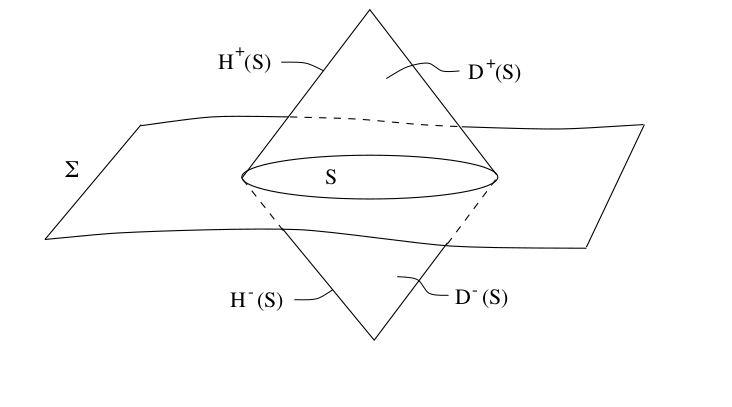
\includegraphics[width=0.7\linewidth]{gfx/CauchyHorizonsGR}
 	\caption{}
 	\label{fig:cauchyhorizonsgr}
 \end{figure}
 
 
 (not necessarily geodesics). We define the \emph{future domain of dependence} of $S$, denoted
 $D_+ (S)$, as the set of all points $p$ such that every past-moving, timelike or null, inextendible
 curve through $p$ must intersect $S$. (“Inextendible” just means that the curve goes on forever,
 not ending at some finite point.) We interpret this definition in such a way that $S$ itself is a
 subset of $D_+ (S)$. (Of course a rigorous formulation does not require additional interpretation
 over and above the definitions, but we are not being as rigorous as we could be right now.)
 Similarly, we define the \emph{past domain of dependence} $D_− (S)$ in the same way, but with “past-
 moving” replaced by “future-moving.” Generally speaking, some points in $M$ will be in one
 of the domains of dependence, and some will be outside; we define the boundary of $D_+ (S)$
 to be the \emph{future Cauchy horizon} $H_+ (S)$, and likewise the boundary of $D_− (S)$ to be the
 \emph{past Cauchy horizon} $H_− (S)$. You can convince yourself that they are both null surfaces.
 \\
 The usefulness of these definitions should be apparent; if nothing moves faster than light,
 than signals cannot propagate outside the light cone of any point $p$. Therefore, if every
 curve which remains inside this light cone must intersect $S$, then information specified on $S$
 should be sufficient to predict what the situation is at $p$. (That is, initial data for matter
 fields given on $S$ can be used to solve for the value of the fields at $p$.) The set of all points
 for which we can predict what happens by knowing what happens on $S$ is simply the union
 $D_+ (S) \cup D_− (S)$.\\
 \\
 We can easily extend these ideas from the subset $S$ to the entire hypersurface $Σ$. The
 important point is that $D_+ (Σ) \cup D_− (Σ)$ might fail to be all of $M$, even if $Σ$ itself seems like
 a perfectly respectable hypersurface that extends throughout space. There are a number
 of ways in which this can happen.
 Glossed over Misner space example and Minkowski space example.
 \\
 A final example is provided by the existence of singularities, points which are not in the
 manifold even though they can be reached by travelling along a geodesic for a finite distance.
 Typically these occur when the curvature becomes infinite at some point; if this happens,
 the point can no longer be said to be part of the spacetime. Such an occurrence can lead to
 the emergence of a Cauchy horizon — a point $p$ which is in the future of a singularity cannot
 be in the domain of dependence of a hypersurface to the past of the singularity, because
 there will be curves from $p$ which simply end at the singularity.
 \begin{figure}[h!]
 	\centering
 	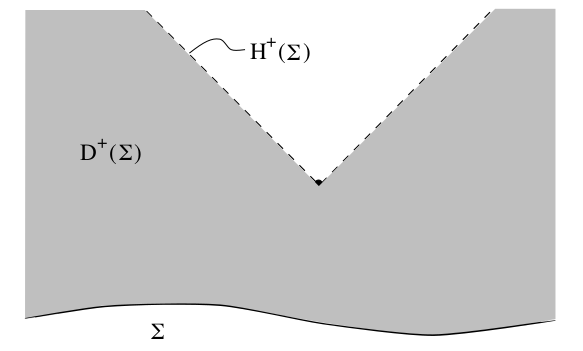
\includegraphics[width=0.7\linewidth]{gfx/SingularitiesGR}
 	\caption{}
 	\label{fig:singularitiesgr}
 \end{figure}
 Singularities are practically unavoidable. The simple fact that the gravitational force is always attractive
 tends to pull matter together, increasing the curvature, and generally leading to some sort of
 singularity. This is something which we apparently must learn to live with, although there
 is some hope that a well-defined theory of quantum gravity will eliminate the singularities
 of classical GR.
 
 
 
 
 
 
 
 
 
 
 \subsection{Hawking-Penrose Singularity Theorems: TO DO}
 \label{subsec:HawkingPenroseSingularity}
 A singularity in solutions of the Einstein field equations is one of two things:\\
 \begin{enumerate}
 	\item
 	a situation where matter is forced to be compressed to a point (a space-like singularity)
 	\item a situation where certain light rays come from a region with infinite curvature (a time-like singularity)
 	Space-like singularities are a feature of non-rotating uncharged black-holes, while time-like singularities are those that occur in charged or rotating black hole exact solutions. Both of them have the property of \emph{geodesic incompleteness}, in which either some light-path or some particle-path cannot be extended beyond a certain proper-time or affine-parameter (affine-parameter being the null analog of proper-time).
 \end{enumerate}
 The Penrose theorem guarantees that some sort of geodesic incompleteness occurs inside any black hole whenever matter satisfies reasonable energy conditions (It does not hold for matter described by a super-field, i.e., the Dirac field). The energy condition required for the black-hole singularity theorem is weak: it says that light rays are always focused together by gravity, never drawn apart, and this holds whenever the energy of matter is non-negative.\\
 \\
 
 Hawking's singularity theorem is for the whole universe, and works backwards in time: it guarantees that the (classical) Big Bang has infinite density.[1] This theorem is more restricted and only holds when matter obeys a stronger energy condition, called the \emph{dominant energy condition}, in which the energy is larger than the pressure. All ordinary matter, with the exception of a vacuum expectation value of a scalar field, obeys this condition. During inflation, the universe violates the dominant energy condition, and it was initially argued (e.g. by Starobinsky[2]) that inflationary cosmologies could avoid the initial big-bang singularity. However, it has since been shown that inflationary cosmologies are still past-incomplete[3], and thus require physics other than inflation to describe the past boundary of the inflating region of spacetime.\\
 \\
 
 It is still an open question whether (classical) general relativity predicts time-like singularities in the interior of realistic charged or rotating black holes, or whether these are artefacts of high-symmetry solutions and turn into spacelike singularities when perturbations are added.\\
 \\
 
 In general relativity, a singularity is a place that objects or light rays can reach in a finite time where the curvature becomes infinite, or space-time stops being a manifold. Singularities can be found in all the black-hole spacetimes, the Schwarzschild metric, the Reissner–Nordström metric, the Kerr metric and the Kerr–Newman metric and in all cosmological solutions that do not have a scalar field energy or a cosmological constant.\\
 \\
 
 One cannot predict what might come "out" of a big-bang singularity in our past, or what happens to an observer that falls "in" to a black-hole singularity in the future, so they require a modification of physical law. Before Penrose, it was conceivable that singularities only form in contrived situations. For example, in the collapse of a star to form a black hole, if the star is spinning and thus possesses some angular momentum, maybe the centrifugal force partly counteracts gravity and keeps a singularity from forming. The singularity theorems prove that this cannot happen, and that a singularity will always form once an event horizon forms.
 \\
 \\
 In the collapsing star example, since all matter and energy is a source of gravitational attraction in general relativity, the additional angular momentum only pulls the star together more strongly as it contracts: the part outside the event horizon eventually settles down to a Kerr black hole (see No-hair theorem). The part inside the event horizon necessarily has a singularity somewhere. The proof is somewhat constructive – it shows that the singularity can be found by following light-rays from a surface just inside the horizon. But the proof does not say what type of singularity occurs, spacelike, timelike, orbifold, jump discontinuity in the metric. It only guarantees that if one follows the time-like geodesics into the future, it is impossible for the boundary of the region they form to be generated by the null geodesics from the surface. This means that the boundary must either come from nowhere or the whole future ends at some finite extension.\\
 \\
 
 An interesting "philosophical" feature of general relativity is revealed by the singularity theorems. Because general relativity predicts the inevitable occurrence of singularities, the theory is not complete without a specification for what happens to matter that hits the singularity. 
 
 
 
 
 
 
 
 
 
 
 
 
 
 
 
 
 
 
 
 
 
 
 
 
 
 
 
 
 
 
 
 
 
 
 
 
 
 
 
 
 
 
 
 
 
 
 

